\documentclass[final, twoadvisors]{nddiss2e}
              % draft + 10pt/11pt/12pt + twoadvisors + textrefs
              % review + noinfo + twoadvisors + textrefs
              % final + noinfo + twoadvisors + textrefs

\usepackage{gensymb}
\usepackage{siunitx}

\newcommand{\nuc}[2]{${}^{#1}\textrm{#2}$}
\newcommand{\mnuc}[2]{{}^{#1}\textrm{#2}}
\newcommand{\react}[4]{$#1(#2,#3)#4$}
\newcommand{\mreact}[4]{#1(#2,#3)#4}
\newcommand{\alpa}{\react{\mnuc{27}{Al}}{\textrm{p}}{\alpha}{\mnuc{24}{Mg}}}

\begin{document}

% Everything before first chapter goes here
\frontmatter

\title{SOME TITLE}
\author{Michael Thaddeus Moran}
\work{Dissertation}
\degaward{Doctor of Philosophy}
\advisor{Mano\"{e}l Couder}
\secondadvisor{Michael C.\ F.\ Wiescher}
\department{Physics}

\maketitle

\begin{abstract}
    The St.\ George recoil separator is currently undergoing its final
    commissioning work to fully characterize it ahead of the first experimental
    campaign to study $(\alpha,\gamma)$ reactions of astrophysical interest.
    The work currently completed to that end and comparison to the expected
    operation will be discussed. A single campaign utilizing the first two
    main sections of St.\ George to study two strong resonances in the
    \alpa{} has been completed as an initial test of the combined angular and
    energy acceptance of th separator, the rejection properties of the Wien
    filter, and the exploration of the use of St.\ George for studying other
    astrophysically important reaction types. The results and comparison to
    accepted values will be presented alongside the extensions to other
    reactions and considerations for extending the analysis capabilities of the
    separator.

\end{abstract}


\begin{dedication}
To Laura, my rock.
\end{dedication}

\tableofcontents
\listoffigures
\listoftables

% \begin{acknowledge}

I would like to thank my advisor, Dr.\ Michael Wiescher, for assigning me to
the St.\ George project and many others along the way. He was a great help as
I explored and discovered my path in science and in life.
For all of his work and guidance to get St.\ George to where it is now, I would
like to thank Dr.\ Manoel Couder. He was always a resource for questions
about mass separator theory, design, and operation, and the primary guiding
force behind the completion of this work, and a support throughout the
entire process.
I would also like to thank the remainder of my committee, Dr.\ Daniel Bardayan
and Dr.\ John LoSecco, for guiding me through the candidacy and defense
process.

The entirety of this project would be impossible without the excellent support
I had throughout the Nuclear Science Lab and the Department of Physics.
In particular,
Dr.\ Daniel Robertson
and Dr.\ Edward Stech were invaluable for learning standard operating
procedures throughout the lab, especially with the accelerators, targets, and
detector systems, and how to be a graduate student within the NSL.
Thank you to Jerry Schur, both for helping me with every network problem that
I happened to forget the solution to at precisely the wrong time.
Thank you to the amazing work done both within and without the machine shop
from
Dave Futa,
Jerry Lingle,
Bradley Mulder,
and Matt Sanford. There have been more times than I could count where this
project would not have moved forward without you.
Thank you to the excellent support from
Susan Baxmeyer
and Shari Herman, who never failed to cheer me up when I saw them in the office
and who helped me navigate through the parts of graduate school life that I had
no idea of what to do otherwise.

Thank you to the greater St.\ George group, past and present\textemdash{}
Dr.\ Manoel Couder,
Dr.\ Jerry Hinnefeld
Dr.\ Zach Meisel,
Gwen Gilardy,
Patricia Huestis,
Edward Lamere,
Luis Morales,
Shane Moylan,
and Chris Seymour\textemdash{}for being the support for when tuning went
poorly and the source of jubilation when things went well. To those future
graduate students and postdocs within the group, I thank you for taking this
project on your own shoulders, and I hope this is a decent starting point for
your own work.

Thank you to
Will Bauder,
Stephanie Lyons Blyth,
Matt Bowers,
Hyu Soon Jung,
Wenting Liu,
Alex Long,
Karen Ostdiek,
Karl Smith,
Kiana Setoodhar,
and Ethan Uberseder,
my former group mates, co-graduate students, office mates, and guiding
older scientists, for helping me as I struggled to figure out who I was as a
scientist and for helping me when the work of physics became too much.

To those close friends that I've made in graduate school\textemdash{}
Will Bauder,
Clark Casarella,
Jared Coughlin,
Edward Lamere,
Charlie Mueller,
Michael Planer,
Jacee Rohlk,
Alicia Spect,
MacKenzie Warren,
and Chris Wotta\textemdash{}thank you for everything. You've each impacted my
life in so
many different ways that listing everything out would triple the length of this
dissertation. You are better than I could have imagined as the people going
through this process with me.
Thank you to Pokie and Mike Olsen, for allowing a young graduate student into
your home and for reawakening my love of board games. I can barely remember a
time before I had to struggle to pay for a 6-cost development, and I didn't
fully appreciate how amazing it was until you left.
Thank you to Kate Turk, for helping me survive graduate school in more ways
than one. You\textemdash{}and of course, your dog Maxwell\textemdash{}have done
so much for me, and I don't think I could ever come close to repaying you.
Thank you again to MacKenzie Warren, who deserved his own mention, for being
the sounding board of my thoughts and feelings
from our time together as roommates through the present day. You've shown me
that people can survive graduate school and come out better from it.
Thank you also to all of those within my graduate cohort and in the physics
department as a whole that I met, joked with, confided in, or just had a good
time with. Your names are far too numerous to list here.

Thank you to my friends from Michigan State, Nichole Hoerner, Gregory Klein,
Christopher Schuster, and Ashleigh Winkelmann. Our continued friendship over
the years has made me realize how lucky I was to stumbled into your lives.

Thank you to my family\textemdash{}my parents, Mike and Brigette, my sisters
Caitlin and Colleen, and my brother Patrick\textemdash{}for always being there
to bring a smile back onto my face during holidays and family trips to the
cider mill. You have shaped me so much as a person during my life, and I know
that I am the person I am now because of how amazing you are as a family.
Thank you also to my extended family, scattered across the states and sometimes
the world as they are, for keeping me in check when I thought to highly or
lowly of myself and my life.

Thank you to Link, for being the derpy sunshine at the end of my graduate
career and for allowing me to laugh at your antics both in the apartment and
outside of it.

Finally, I would like to thank my wife, Laura Amelia, for being there. When you
entered my life during my first year of graduate school, I could not have
predicted to drastic positive change you made in my life. You have gotten me
through graduate school in more ways than one, and I could not have done all of
this without you by my side. While this part of our lives is now over, I am
excited to begin our next stage together as we leave Notre Dame behind. I love
you with all of my being, and I thank you for sticking with me.

\end{acknowledge}


\begin{dedication}
Your confusing thesis has captured my attention. Tell me more.
\newline\---{} Phil Hartman as Bill McNeill (Newsradio)
\end{dedication}

% All main text goes here
\mainmatter
\chapter{INTRODUCTION}

The elements making up the universe were formed during a variety of processes,
beginning with Big Bang Nucleosynthesis (BBN) that formed the lightest
elements. Those elements common to life on Earth were primarily formed through
burning processes inside of stars, grouped together under the title of
Stellar Nucleosynthesis. Depending on the conditions within the stellar
environment, which are characterized by macroscopic qualities about the star
(temperature, pressure, mass, etc.) and the elemental composition of the
stellar interior where the burning process takes place, the reactions
accessible to the nuclei within the star differ. The creation and destruction
of different elements and isotopes may be inhibited or enhanced by these
differing conditions, and the study of these processes at the nuclear level
has spawned the field of nuclear astrophysics in order to understand the inner
workings of these stars.

The study of these reactions has increasingly taken place within nuclear
accelerator laboratories, which can attempt to replicate the conditions inside
of stars in order to measure the qualities of the reactions as they take place
in the cosmos. Individual reactions may be isolated by the choice of the
accelerated beam particle and its properties, and the choice of target material
and its properties. As the underlying cross section governing the observed
properties of the reaction may change rapidly within a narrow band of energy,
immense amounts of work and effort has been expended in order to detect these
changes with enough precision in order to be confident that the cross section
has been accurately described. Whole classes of reactions and detection methods
have been devised to study those reactions previous out-of-reach to experiment,
either due to the energies in question or the complexities of detecting the
desired particles.

In order to properly measure a single cross section, a [COMPLETE?] knowledge of
the relevant physical processes and experimental methods is paramount. The
astrophysical motivation for studying certain reactions and the experimental
techniques devised to study these reactions will be explored.

% some more lead-in...?


\section{Astrophysical Reaction Channels}
\label{sec:ch01-astrophysical-reaction-channels}

The specific and directed study of those nuclear reactions that have an effect
on the properties or life cycle of celestial bodies is grouped under the
umbrella term \emph{nuclear astrophysics}. These reactions may take place
during the standard lifecycle of a star, called \emph{stable burning}
processes; during the death throws of a star, called \emph{explosive burning}
processes; or during the grander timeline of the universe as a whole, among
other coarse groupings of reactions. A more-complete exploration of these
aspects of nuclear astrophysics was first laid out in [B2FH].

Within the realm of stable burning processes, changes in temperature commonly
result in reaction channels or sequences becoming either energetically
favorable or unfavorable.

The two primary reactions that will
be discussed, \alpa{} and \nag{},
are important reactions in a number of different reaction chains that take
place throughout the lifecycle of stars, and the impact of these reactions will
be explored.

\subsection{Hydrogen Burning}

Hydrogen burning is the net fusion of four protons into a single Helium
nucleus. Stable hydrogen burning is the process wherein the reaction chains
involved take place within a star during its regular lifecycle.

\subsubsection{$pp$ Chain}

Stars similar to our Sun fuse hydrogen through the $pp$ chains, which are
described by the reaction sequences
\begin{align*}
    \rm{PP-1}& \mreact{\rm{p}}{\rm}{e^+\nu_e}{\mnuc{2}{H}} \
    \rm{PP-2}& \
    \rm{PP-3}&
\end{align*}
The net effect of these reaction sequences is the reaction
\[
    4\rm{p} \rightarrow \mnuc{4}{He} + 2e^+ + 2\nu_e,
\]
with the primary difference being what intermediate nuclei the reaction
progresses through. Each of the identified $pp$-chain sequences releases the
same amount of energy (XXX MeV) and become energetically favorable in different
temperature ranges inside of stars.

\subsubsection{CNO Cycle}

The Carbon-Nitrogen-Oxygen (CNO) cycle is an additional pathway for stable
hydrogen burning making use of catalytic nuclei to produce \nuc{4}{He} through
the reaction sequences
\begin{align*}
    \rm{CNO-1}& \mreact{}{}{}{} \
    \rm{CNO-2}&
\end{align*}
The CNO cycles dominate the energy production of heavy stars with properties
[MASS and TEMPERATURE].

\subsection{$s$-Process Nucleosynthesis}

- end state of CNO is more 14N than anything else
- Breakout reaction feeds into s-process by generating seed nuclei
- s-process progresses in AGB stars over long timescales
- produces high mass nuclei near the valley of stability

\subsection{Other Channels...?}

- where does 27Al(p,a) fit in?
- hydrostatic hydrogen burning in AGB stars
- explosive hydrogen burning in a nova
- np-process, sp-process, r-process, etc?


\section{Recoil Mass Separation}
\label{sec:ch01-recoil-mass-separation}

When measuring a cross section, the experimenter must make a decision as to
whether to detect $\gamma$-ray particles or nuclear particles. Each of these
two overarching goals carries with it their own complications and
considerations, creating a variety of techniques to attempt to study the
reaction in question. For some reactions of interest within the domain of
low-energy nuclear astrophysics, both or these experimental directions are
possible.

Gamma-ray detection suffers from background radiation producing $\gamma$ rays
that are picked up by the detector. This background radiation is produced by
the construction materials within the laboratory in question, cosmic radiation,
and the $\gamma$-ray producing reactions involving contaminants within the
target material. The solutions for reducing the background from each of these
sources are varied, from surrounding the detector with additional detectors to
create an active shield that rejects detections that appear in both detectors
within some window of time (the anti-coincidence method), to the extreme case
of placing the laboratory deep underground to use hundreds of meters of the
Earth's crust as a passive shield against cosmic radiation. None of the
techniques, however, addresses the inherent limitation of $\gamma$-ray
detection: the low efficiency of the detectors that must be used. This problem
is exasperated by the extremely low cross sections common for reactions of
astrophysical interest, making studies away from nuclear reasonances uncommon.
The other irreducible problem with these techniques is when the produced
$\gamma$ ray of interest is close in or the same energy as a prominent
background line.
%, such as the 511~keV $e^+e^-$ annihilation peak.

Alternatively, the produced nuclear particles may be detected instead with a
high-efficiency detector. The various experimental requirements for these
experiments will be discussed, along with the additional considerations that
must be accounted for. For convenience, the rest of this discussion will assume
that the reaction of interest is radiative alpha capture ($(\alpha,\gamma)$),
where the reaction is being studied in reverse kinematics, except where
otherwise noted.

% This previous paragraph is weird... I'm not sure how to transition here

St. George (Stong Gradient Electromagnetic Online Recoil separator for capture
Gamma ray Experiments) is a recoil separator designed to primarily study
$(\alpha,\gamma)$ reactions at low energy using stable beams provided by St.
Ana (Stable beam Accelerator for Nuclear Astrophysics). The design of the
separator was guided by the principles to be discussed and on the experience
gained from previous recoil separators.


\subsection{Motivation}

Recoil mass separation was conceived as an alternate way to measure the cross
sections of radiative capture reactions. These reactions had previously been
studied by detecting the produced $\gamma$ rays, subject to the limitations
previously discussed. The heavy reaction product can instead be detected by a
detector situated behind the target, assuming that the target is thin enough to
allow the produced recoils to leave the target. In this thin target case, the
incident beam will likely pass through the target as well, making it a source
of background at the detector plane. In the cases of interest for nuclear
astrophysics, this background count rate could be $\times 10^{15}$ that of the
particles of interest and may cause damage to the detector.

The produced recoils may be filtered out from the incident beam by
electromagnetic elements situated between the target and the detector. The
interaction between the heavy incident beam with mass $A$ and linear momentum
$p$ and the $\alpha$ particles within
the target produces a heavy compound nucleus with mass $A + 4$ and momentum
$p$. Ignoring the effect of the emitted $\gamma$ ray on the momentum and
assuming that there is no spread in the momentum, the use of electrostatic
elements can separate the recoils from the beam based on their different
magnetic and electric rigidities, defined as
\[
    B\rho\,\rm{[Tm]} = \frac{p}{q} = \frac{\sqrt{2mT}}{q}
\]
and
\[
    E\rho\,\rm{[MV]} = \frac{pv}{q} = \frac{2T}{q},
\]
respectively, where $q$ is the charge, $T$ is the kinetic energy, $m$ is the
mass, and $v$ is the velocity of the particle. With a single momentum and
velocity (or kinetic energy) selected for, the recoil particles of interest can
be uniquely identified by the optical system. The design of recoil separators
make use of this relatively simple idea as the basis of their design. Despite
this, there have been relatively few recoil separators that have been brought
into service due to the complexities of their design and operation that are not
adequately taken into account in this description.


\subsection{Background Sources}

A recoil separator primarily utilizes two different methods to reduce the
background at the detector system: the separation of isotopes based on their
rigidities to reduce the number of incident beam particles that reach the
detector, and the direct detection of the heavy nuclear particles compared to
the detection of the $\gamma$ rays particles produced in the reaction at the
target location. These reduction techniques have been briefly introduced.

Within the separator, the rejected incident beam particles (those which do not
have the desired rigidities $B\rho$ and $E\rho$) are still traveling within
the separator. Their final rejection and the reduction of their induced
background at the detector plane must be performed by some physical element
interior to the separator. A common choice of element are slits: physical
barriers that stop any particle which strikes them located within the
separator. The physical gap between the slits allow the desired recoil
particles to pass between them while stopping the unwanted beam particles from
continuing down the separator. The location of these slits is dependent on the
design and the beam optics of the separator.

While these slits stop errant beam particles, there is a possibility of those
particles scattering off of the edge of the slit if the beam properties are
not properly matched to the internal position or gap of the slits. These
scattering events, depending on where in the separator they occur in relation
to the other magentic and electric elements and to the detector system, may
allow some passage of beam particles to the detector plane and must be either
rejected before that plane or taken into account in the operation of the
detector system. The scattering events may also take place off of the interior
of the vacuum chamber of the separator, the residual vacuum within the vacuum
chamber, or diagnostic equipment installed to aide the experimenter.

The reaction also does not take place at a single energy. The incident beam
invariably will have an energy spread associated with its production and will
lose energy within the target before reacting with the target particles. The
produced reaction products will necessarily not be mono-energetic, and
additional energy spread will result from the subsequent interaction with the
residual target. The reaction products also undergo either a single photon
emission or a gamma cascade which will alter the reaction products' momentum
vectors, adding futher spread to the momentum and energy of the products that
must be detected at the detector plane. Additional sources of background
reduction beyond the separator must be included due to the realities of
performing the experiment.


\subsubsection{Detection System}

The detector system following the separator may be used to provide this
additional required beam and background suppression. Due to the separation of
the recoil particles by their rigidity, a detector sensitive to both the energy
and the momentum of the particles can unique identify those particles. There
are multiple ways in which this can be achieved, but one common design is to
make use of a \textit{time-of-flight} (TOF) detector to determine the velocity
of the particles reaching the detector, and an energy-sensitive detector,
measuring the total energy deposited in the detector, to provide this
identification. Depending on the resolutions of the two systems, the recoils of
interest can be identified by the recorded TOF and $E$. More importantly, those
other particles that happen to reach the detector would have drastically
different TOF or $E$ or both, allowing those detections to be rejected as they
did not originate from recoil particles.

The two coupled detectors would be operated in coincidence, such that those
events that create a timing signal within the TOF detector must also create an
energy signal in the following energy-sensitive detector in order for the
event to be recorded. This operation further suppresses errant background
counts at the detector system. The timing window must be matched to the
properties and response of the detectors in order to ensure that the
coincidence measurements from the paired detectors arise from a single
particle.


\subsection{Recoil Separators}
\label{sec:ch01-recoil-separators}

% The implementation of recoil separation into experimental campaigns has been
% explored recently at a number of facilities, primarily with a focus on studying
% astrophysically relevant reactions. When considering each separator facility and
% the capabilities of that system, the separator must be considered alongside the
% target, detector, accelerator, source, and other essential elements within the
% entire laboratory.
% St.\ GEORGE (Strong Gradient Electromagnetic Online Recoil separator for
% capture Gamma ray Experiments, henceforth simply \emph{St.\ George}), is one
% recent recoil separator, installed at the Nuclear Science Laboratory (NSL)
% at the University of Notre Dame~\cite{Couder2008}.
% The design for St.\ George is based on knowledge gained by
% designing, constructing, and using these previous
% separator systems for scientific research.
% Where these systems are similar and
% differ from the system in place at the University of Notre Dame will be briefly
% discussed. Additionally, a brief description of the St.\ George separator will
% be included here and further discussed in Sec.~\ref{sec:stg}.

The use of recoil separators to study radiative capture reactions has been
explored recently at a number of facilities. The design of St. George is based
on the knowledge gained from the design, construction, and operation of these
previous recoil separator systems. The entire system, inclusive of the beam
source, target, and detector, must be discussed as a whole when evaluating the
capabilities of a given separator.


\subsubsection{CalTech Separator}

% The design and use of recoil separators for astrophysical studies was first
% pursued by Smith \textit{et al.}~\cite{Smith1991}. The requirements of radioactive
% beam studies required the need to develop new detection systems, especially
% considering the effect of differing beam property limits (intensity, purity,
% and emittance) and the desire to detect the produced nuclei to further probe
% the astrophysical conditions. As the initial feasibility system to provide a
% technical proof-of-concept, many of the design choices made and techniques
% used have been adopted by following separators. These include the use of a Wien
% filter for velocity selection, dipole magnets for momentum selection, an
% electrostatic deflector for energy selection, and the use of a gaseous target.
% Additionally, the use of a gamma-ray detector in coincidence with the final
% recoil detection and beam monitoring with an offset Si detector at the target
% location are also common choices that have been adapted at the other separators.

The design and use of recoil separators for nuclear astrophysics research was
pioneered by Smith *et al.*. This separator was a proof-of-concept design to
determine the feasibility of performing reaction studies with this technique.


\subsubsection{ARES}

The Astrophysics REcoil Separator (ARES) was built at Louvain-la-Neuve to
study $(\rm{p},\gamma)$ and $(\alpha,\gamma)$ reactions using radioactive
incident beams provided by the CYCLONE44 cyclotron~\cite{Angulo2001}.
Self-supporting solid
targets, containing the required H or He, were used for the reaction
studies. The system is designed with a single magnetic dipole for momentum
selection and a Wien filter for velocity selection, along with multiple
magnetic quadrupoles to maintain the transportation of the to the detector
system. The condensed and limited size of the separator is based on the
constraints of the experimental hall~\cite{Couder2003}.
The detector system consists of a single
$\Delta E − E$ telescope which separates out the reaction products from the
remaining incident beam particles. The initial test of the separator used a
stable incident beam to compare to results obtained by other methods within
the lab, and the focus of the initial work was on low-lying resonances of
astrophysical interest.


\subsubsection{DRAGON}

The DRAGON recoil separator at TRIUMF-ISAC was built for the same reasons as ARES,
but differs in the actual construction and usage of the separator.
% Success of separator
The separator
itself uses two large magnetic dipoles for momentum separation and to electric
dipoles for energy selection~\cite{Engel2005}. The separator also contains
steering elements within the beamline to aide in transporting the recoils to
the detector plane. The extended gas target is surrounded by a large BGO
gamma-ray detector for coincidence purposes

\subsubsection{ERNA}

% Look up ERNA design/commission paper(s)
The ERNA (acronym) recoil separator at (location)...


\subsubsection{St. GEORGE}
The separator consists of six dipole magnets, eleven quadrupole magnets, and a
Wien filter. The separator was designed to accept recoils with a maximum
energy and angular spread of $\Delta E/E = \pm7.5\%$ and
$\Delta\theta = \pm40$~mrad, respectively, and to provide a mass separation
of $m/\Delta m = 100$ and beam suppression of a factor $\geq 10^{15}$. Combined
with the HIPPO (High-Pressure Point-like target) supersonic gas jet target,
St.\ George will be primarily used to study low energy $(\alpha,\gamma)$
reactions using stable beams.



\section{Beam Optics}

% quadrupole and dipole fields...?

The understanding of how recoil separators work is grounded in the theory of
beam optics which describe the effect of electric and magnetic fields on moving
charged particles. These moving particles are focused and directed by the
electromagnetic elements, and their action on particles can be modeled and
optimized to transport particles with various properties down a beam line to a
desired location.

- parts of beam optics?
- Louisville theorom (conservation of phase space)
- connection to properties (resolution?)
- references to code/COSY?

\chapter{EXPERIMENTAL SETUP}
\label{ch:commissioning}

% REORG: STG and commissioning work separate out better

All experimental work was performed at the Nuclear Science Laboratory (NSL) at
the University of Notre Dame, using the St.\ Ana 5U-4 accelerator and
St.\ George. Commissioning work for the separator began in 2014 and is
currently on-going (see Section~\ref{sec:commissioning}). The experiment discussed
herein consisted of three separate runs, each one week long, in December 2016
and February 2017. The first run tested a proposed close location for the
detection system, the second run characterized the additional magnets required
for a far location for the detection system, and the third run was the primary
data collection run.

The accelerator provided a high intensity proton beam to St.\ George for the
first and third runs, and a high intensity $\mnuc{4}{He}^{+}$ beam for the
second characterization run. The 16-strip Si detector was installed at the two
proposed focal planes ($F_1$ and $F_2$, see Fig.~\ref{fig:stgeorge}) to detect
the produced $\alpha$-particles from the \alpa{} reaction. Incident beam
rejection was on the order of $10^9$ for the first run and $10^{13}$ for the
third run [CHECK THESE NUMBERS].


\section{The St.\ Ana Accelerator and Transport Line}
\label{sec:5U}

St.\ ANA (Stable beam Accelerator for Nuclear Astrophysics) is a 5~MV vertical,
single-ended pelletron accelerator at the NSL, providing high-intensity stable
beams to a number of experimental setups within a dedicated target room. The
original designation of the accelerator by the manufacturer, National
Electrostatics Corporation, was the 5U-4, denoting the five individual
acceleration sections and the four charging chains, causing the accelerator to
commonly be referred to as the \textit{5U}. Both names will be used
interchangeably throughout this work.

The 5U, shown schematically in [FIGURE], accelerates a high-intensity ion beam
produced by the Nanogan Pantechnik ECR source to the desired energy by
energizing the
terminal shell to high voltage. The acceleration tube, extending from the
bottom of the shell to the bottom of the accelerator, steps that voltage down
through a series of resistors and plates, creating an electric field gradient
along the tube that accelerates the positively charges ion beam down and out of
the accelerator. The beam is then bent around a 90\degree dipole magnet, called
the analyzing magnet, and through a pair of vertical slits, called the
analyzing slits, that provide energy identification of the beam.
In addition, the
current on the slits can be used as a feedback control system to regulate the
voltage on the terminal shell when the accelerator is being run in ``slit
control mode,'' providing a highly stable beam with a small energy spread.
A recently performed \react{\mnuc{27}{Al}}{\textrm{p}}{\gamma}{\mnuc{28}{Si}}
resonance scan~\cite{Gilardy2017} was used to determine the beam energy spread
of $\sigma_{\textrm{beam}} \approx 0.3$~keV near a beam energy of
$E_{\textrm{beam}} = 1320$~keV. The 5U also contains
focusing, directional, and diagnostic elements used to help tune the accelerator
to provide a stable and well-behaved beam.

The transport beamline directs the analyzed beam to the desired
experimental area through use of focusing and directional elements: two
magnetic
quadrupole doublets maintain a focused beam along the beamline; the magnetic
dipole switching magnet
directs the beam down one of the available experimental beamlines; and magnetic
steerers shift and turn the beam within the beamline. The steerers act to
maintain the beam along
the magnetic optical axis of the quadrupoles and maximize the amount of beam
being transported down the beamline from
the accelerator. Sets of diagnostic equipment are also installed at various
locations along the beamline to help monitor and restrict the beam, and the
entire system is kept at a high ($\approx 8\times 10^{-8}$~torr) vacuum through
use of multiple turbomolecular pumps located along the beamline.

The final section of the transport line is between the switching magnet
and the entrance to St.\ George.
This section of beamline prepares the beam to have the required characteristics
at the target location. The final magnetic steerer is used to finalize the
alignment of the beam, and the magnetic quadrupole triplet creates a small,
well-focused beam at the target location.


\section{The St.\ George Recoil Separator}
\label{sec:stg}

The St.\ George is a
recoil mass separator at the NSL~\cite{Couder2008} and one of the experimental
beamlines accessible to the 5U. The design and operation is based on
previous recoil separators (see Sec.~\ref{sec:prevwork}). The separator
consists of six dipole magnets, eleven quadrupole magnets, and a Wien filter.
The separator was designed to accept recoils with a maximum energy and angular
spread of $\Delta E/E = \pm7.5\%$ and $\Delta\theta = \pm40$~mrad,
respectively, and to provide a mass separation of $m/\Delta m = 100$ and
beam suppression of a factor $\geq 10^{15}$. At lower angular spreads, the
transported ions may have a larger energy spread limited by the good field
region within the third quadrupole $Q_3$. The design was guided by the desire
to efficiently measure $(\alpha,\gamma)$ reactions with a beam mass up to
$A = 40$ with high beam intensities and to fit the separator within the
physical limitations of the target room at the NSL~\cite{Couder2008}.

The separator is designed to transport recoils within a rigidity phase space
relevant for measuring $(\alpha,\gamma)$ reaction cross sections, determined by
the magnetic and electrostatic elements. The magnetic rigidity is defined as
\begin{equation}
    \label{eq:brho}
    B\rho\textrm{ [Tm]} = \frac{p}{q} = \frac{\sqrt{2mT}}{q},
\end{equation}
where $p$, $q$, $m$, and $T$ are the momentum, charge state, mass, and kinetic
energy of the desired particle, respectively. The magnetic rigidity
defines the trajectory of the particle's movement within a homogeneous magnetic
field of strength $B$ along a circular path with radius $\rho$. Similarly, the
electric rigidity is defined as
\begin{equation}
    \label{eq:erho}
    E\rho\textrm{ [MV]} = \frac{pv}{q} = \frac{2T}{q}
\end{equation}
with the same variable definitions as before, and defines the circular
trajectory a particle takes within an electric field of strength $E$. The
limits for these rigidities are $0.1 \leq B\rho \leq 0.45$ and
$E\rho \leq 5.7$~\cite{Couder2008}.


\subsection{Subsections of St.\ George}

\begin{figure}[t]
    \begin{center}
        \centerline{\includegraphics[width=0.95\textwidth]%
            {figures/st_george.png}}
        \caption[Layout of the St.\ George recoil separator]{Layout of the St.\
            George recoil separator. Quadrupoles are identified by $Qn$,
            dipoles by $Bn$, and focal planes by $Fn$. Section labels are
            placed near the dipole doublet within that section, and boundaries
            are the intervening focal planes. Adapted from
            Reference~\cite{Couder2008}.}
        \label{fig:stgeorge}
    \end{center}
\end{figure}

The separator is divided into three sections, based on their purpose: the
charge selection stage; the mass selection
stage; and the clean-up stage. The stages are separated by the focal planes.
Each of these stages will be discussed in turn. The layout of
St.\ George is shown in Fig.~\ref{fig:stgeorge}.

The entire separator is tuned for a single $B\rho-E\rho$ rigidity, defined by
the central energy of the recoils and its mass and charge state (see
Eqs.~\ref{eq:brho} and \ref{eq:erho}). For commissioning purposes, a direct
incident beam was used as a ``test beam'' to tune the separator without having
to perform a reaction. The tuned particles will then travel down the central
magnetic axis of the separator. Particles that differ in energy or angle from
these central particles will travel through a different path (see
Fig.~\ref{fig:raytrace}).

The first section is the so-called \textit{charge selection} stage, consisting
of the
first quadrupole doublet ($Q_1Q_2$) and the first dipole doublet ($B_1B_2$).
The doublet $Q_1Q_2$ focuses the recoils through the dipole pole gap, and the
doublet $B_1B_2$ provides the first rejection of beam due to the difference in
magnetic rigidity from the desired recoils. At the first focal plane $F_1$, a
single recoil charge state has been selected to transport through the remainder
of the separator. Horizontal slits may be placed at this focal plane to aide in
the rejection of incident beam particles that have undergone a charge exchange
event. Slits were not used during the commissioning work or during the primary
experiment. At the end of this section, both beam and recoil particles are
present within the separator.

The next section is the so-called \textit{mass selection} stage, which contains
the
magnetic quadrupole triplet ($Q_3Q_4Q_5$), the second magnetic dipole doublet
($B_3B_4$), the second magentic quadrupole doublet ($Q_6Q_7$), and the Wien
Filter (WF). This section's primary purpose is to reject the incident beam and
create an achromatic focus at the second focal plane $F_2$. This focus is
horizontally narrow at the focal plane to aide in the rejection of the beam.
At this focal plane, a set of horizontal slits, called the mass slits,
are placed to reject the remainder of the incident beam. The focused recoil
particles will pass through the center gap between the slits. The mass
resolution of the separator depends on the particle distributions of the beam
and recoil being focused and spatially separated at this position, and that the
tail of the beam distribution minimally overlaps with the recoil distribution.

The Wien filter operates by having crossed electric and magnetic fields,
oriented such that individually they would bend a particle beam in opposite
horizontal directions, as shown in Figure [FIGURE]. From the beam's
perspective, the electric field bends the beam to the right while the magnetic
field bends the beam to the left. The fields are provided by a pair of
electrostatic plates within the vacuum chamber and a magnetic dipole outside of
the chamber. A Wien filter is set to allow for a single velocity to pass
through the center of the element undeflected, according to $v = E/B$. For
St.\ George, the Wien filter provides the final mass selection for our recoils,
allowing the beam particles to be filtered out from the recoil particles, since
the mass difference between the two ($\Delta m = 4$ when performing
$(\alpha,\gamma)$ reactions) translates into a velocity difference.

The simplified description above is not entirely accurate, since our beam and
recoils exist within a phase space envelope confined by ranges of allowed
positions, angles, and energies. Since we inherently have an energy
distribution of our recoils deriving from the convolution of the beam energy
uncertainty with the target losses of the beam and recoils and the energy
change arising from the $\gamma$ ray emission, we do not have a mono-energetic
recoil distribution passing through the center of the WF. When taken as a
whole, the elements up to and including the WF create the proper beam and
recoil properties to reject the incident beam based on their mass difference.

At this point, our beam envelope can be thought of as just our \textit{recoil}
envelope, where the particles still being transported through St.\ George are
just those recoils produced in the reaction at the target location. In reality,
the envelope still contains some beam particles, either through scattering off
of the interior of the beam pipe, diagnostic elements, or the residual vacuum,
or through charge changing events with the residual vacuum [CITE]. Due to these
factors, we cannot place the final detection system right after the Wien
filter and instead need additional elements to further reduce the background.

This final section of St.\ George is the so-called \textit{clean-up} stage,
where the phase space of the recoils passing through the mass slits are matched
with the phase space of the detection system, providing the last rejection of
the incident beam particles. This section consists of, in order, a quadrupole
doublet ($Q_8Q_9$), the last dipole doublet ($B_5B_6$), and a final quadrupole
doublet ($Q_{10}Q_{11}$). These magnets transport the recoil particles that
passed through the mass slits at $F_2$ through the detection system installed
at the detector focal plane $F_3$. Since the detection system has a defined
physical acceptance size, these magnets must reduce the physical extent of the
recoil envelope within this space.


\subsection{Diagnostic Equipment}
\label{sec:diagnostic}

To aide tuning the beam, additional diagnostic equipment has been developed and
installed at various points along the separator. This diagnostic equipment can
be divided between three basic types: Faraday cups, slits, and quartz viewers.
These first two equipment types are present within other beamlines and the
primary transport beamline, while the third was adapted for St.\ George based
on principles encountered when working with other beamlines. The positions of
this equipment is denoted in Figure [FIGURE].

Faraday cups are beamstops that also provide the user with the beam current
being captured by the cup. The cup, shown in [FIGURE], consists of three main
parts: the shield, the suppression, and the cup itself. This structure is
attached to a linear motion drive, letting the cup be positioned in or out of
the beam, and isolated from the beamline. The shield primarily protects the
suppression from being hit by incident beam but, due to its isolation, is also
a point to read out the current and determine the physical extent of the beam
at that point. Ideally, all of the beam would enter the cup portion, allowing
the Faraday cup to determine the complete beam current at that location. Using
the cup in this way as a tuning aide is possible since the cup locations were
selected based on the beam optics properties, as those locations
correspond to waist points of the beam. The suppression is necessary since
electrons are emitted with energies in the rough range of $20-100$~eV
when the beam strikes the physical cup. By biasing the suppressor to $-300$~eV,
those electrons are directed back toward the cup, giving an accurate reading of
the beam current actually hitting the cup.

Slits are an additional way to determine the passing beam current but also
provide information about the spatial size of the beam. These slits are Ta
plates attached to a linear motion, allowing the position to be controlled and
determined from the exterior of the beamline. Each slit is isolated from the
beamline, allowing the current hitting the slit to be read out at the console
or to some other diagnostic program. The limiting factors for using these slits
as a diagnostic device is their sensitivity, since unlike Faraday cups the
slits used within St.\ George are not suppressed. The slits are then used as
rough spatial diagnostics within the separator itself.

The quartz viewers used within St.\ George are divided between two types: an
exterior quartz located at various exit ports, and an interior quartz that must
be removed from the beamline. The locations of these camera systems are at the
0\degree{} exit ports of dipoles $B_1$, $B_3$, and $B_5$, the end of the
detector chamber, and at focal planes $F_1$ and $F_2$. A schematic of one of
the interior quartzs is shown in Figure~[FIGURE]. The quartz are used for beam
alignment and tuning the magnetic and electric elements of St.\ George, as
explained in Section~\ref{sec:commissioning}. When beam strikes the quartz
material, the quartz fluoresces and the camera mounted immediately behind
records the image and transmits it to the control console. Since this
fluorescence is dependent on the beam intensity, minimum currents of 200~nA are
used to ensure that the beam shape can be accurately identified. Additionally,
high intensity beams can melt the quartz material if left impinging on the
system for extended periods of time, so maximum currents in the range of
$1.5-2.5$~$\mu$A were used, depending on the actual beam particle selected.


\section{Detector System and Data Acquisition}
\label{sec:detector}

The full St.\ George detector system consists of a pair of microchannel
plate based time-measurement detectors and a single 16-strip Si detector for
energy deposition. Combined, this detection system provides particle
identification by way of the \textit{Time of Flight vs.\ Total Energy}
method. As residual beam particles can make it to the detector plane, either
through scattering or charge exchange events, particle identification is
required to provide final discrimination and beam suppression
[CITE ERNA, DRAGON, DRS, etc]. As this experiment did not require the use of
the full detection system, only the Si detector will be discussed further.

The Si detector is a Canberra PIPS (Passivated Implanted Planar Silicon)
model PF-16CT-58*58-300EB, which has a detector area of $58\times 58$~mm
and is divided into 16 individual strips. The 16 strips allow for spatial
resolution in one dimension, commonly taken to be the horizontal direction.
For the experiment discussed herein, the detector was installed at focal plane
$F_2$. Care was taken to ensure that the quartz viewer at that same location
did not interfere with the operation of the detector.

The electronics for the experiment are relatively simple, needing only the
energy signals from each of the 16 strips. A Mesytec MSCF-16 shaping filter
amplifier provided amplification and signal shaping following the preamplifier,
and a Caen V785 32-channel multi-event peak sensing ADC transformed those
signals for the data acquisition system. Power to the detector was provided by
Mesytec MHV-4 high precision bias supply unit, and was biased up to +40~V.
Leakage current from the detector during the run was $\approx 1.4$~$\mu$A, but
this high value was later shown to be due to the cable shielding internal to
the beamline contacting the shielding installed to protect the detector when
fully retracted. During the energy calibration runs where no detector shielding
was present, the leakage current was $\approx 0.3$~$\mu$A. The electronics used
are the same as for a standard St.\ George experiment, allowing for an
additional test of a subsystem of the full acquisition system. Data was
recorded using the VM-USB crate connected to the St.\ George DAQ
computer.


\section{Target Chamber}
\label{sec:target}

A commissioning target chamber was designed and built specifically for running
the commissioning experiments and solid target studies. The chamber makes use
of two of the turbomolecular pumps from the Hippo target to provide a high
($\approx 7\times 10^{-8}$~torr) vacuum at the beginning of the separator and
around the target location. The commissioning chamber consists of a pair of
electrostatic plates within a rotating chamber, a target ladder, and a Faraday
cup. The rotating chamber allows the combined target ladder and electrostatic
plates to rotate through a range of $\approx 160\degree$ (limited by the
physical space around the target location) while maintaining a high vacuum,
thus the target location does not need to be vented in order to change the
angle of the target ladder and plates.

The electrostatic plates can be powered up to a maximum of 10~kV each from two
single-phase high voltage power supplies and are operated remotely using an
Arduino-based controller. The properties of the plates (length, width,
separation, etc.) were determined such that the produced electric field would
be as homogeneous as possible within the limited space and provide a beam
deflection of at least 40~mrad from the target location, within the physical
limits of the chamber. Experimentally, deflections of 45~mrad have been
achieved, allowing a full angular phase space sweep to be performed. Switching
the polarity of the deflector plates must be done at the power supplies. Since
the power supplies have a limited upper voltage, the maximum deflection for a
test beam is limited by its electric rigidity $E\rho$. When not in use, the
current striking the deflector plates could be monitored at the control console
to use as an additional beam diagnostic.

The target ladder contains a 6.35~mm diameter collimator and a 2.06~mm
collimator, separated by 11.1~mm. The large collimator is primarily used for
mounting self-supporting solid targets, while the smaller collimator is
primarily used for beam alignment and focusing purposes. The ladder is mounted
on a high precision, manually controlled linear motion drive from [COMPANY].
The ladder may be fully removed from the beamline, and the central axis is
aligned with the physical location of the jet target within Hippo. A thin Al
foil was mounted for the experiment described herein.

The Faraday cup following the target chamber is an isolated FN-style cup, as
shown in [FIGURE]. The back of the cup can be actuated open to allow beam to
pass into the separator. From extended usage of the cup, the interior
connection to the rear flap had degraded to the point that when open it was
electrically isolated from the rest of the cup. If actuated while beam was
hitting the cup, the flat would become charged and deflect the beam entering
into St.\ George. To counter this effect, the cup preceding the target cup was
placed into the beam before the target cup was removed. Since the commissioning
chamber was designed to be temporary, this cup was not repaired or replaced
following this discovery.

The Faraday cup allowed for beam with a maximum deflection of $>45$~mrad to
enter St.\ George, as measured using the deflector plates. This larger angular
acceptance at the beginning of the separator ensured that the diagnostic
equipment did not have a detrimental affect on the experiment and based the
final acceptance at $F_2$ to be based on the specific tune of the separator.
During some tests, the deflector plates were seen to intercept some of the beam
when deflecting to 45~mrad, but since this value is again larger than the
designed acceptance of St.\ George, this was deemed to not be detrimental.

\chapter{COMMISSIONING ST.\ GEORGE}

The St.\ George recoil mass separator was designed to have an energy acceptance
of $\Delta E/E = \pm7.5$\,\% and an angular acceptance of
$\Delta\theta = \pm40$~mrad, based on the kinematics of a set of
astrophysically important $(\alpha,\gamma)$ reactions~(\cite{Couder2008} and
Section~\ref{sec:stg}).
% The total acceptance, i.e.\ the combined angular and energy acceptance, must be
% determined experimentally through direct beam studies, simulating reaction
% products with a degrading foil, or actually performing a reaction study.
The ion optics that maximize the acceptance of the recoil particles and the
rejection and suppression of the beam particles must be experimentally
determined. The calculated ion optics are related to those achieved
experimentally through the measured performance of the recoil separator. By
measuring the acceptance achieved through various tunes and techniques is one
way to determine if the desired calculated transport properties have or have
not been achieved experimentally.
Recently, the energy acceptance was initially studied separately from the
angular acceptance (published in \cite{Meisel2017}) to provide a relation
between the predicted and experimentally determined field values. The angular
acceptance was studied through a variety of methods, both in conjunction and
without a corresponding energy acceptance requirement. Measuring the acceptance
of a separator is paramount to using it for experimental measurements.

Two primary commissioning campaigns, determining the angular and energy
acceptances for a given desired global setting of the separator, have been
undertaken. The two global settings are: (i) the designed parameters for St.\
George for transporting heavy recoil products produced by $(\alpha,\gamma)$
reactions in inverse kinematics through the entire separator, and (ii) the
altered parameters for transporting $\alpha$ particles produced by
$(\textrm{p},\alpha)$ reactions in forward kinematics to focal plane $F_2$.
From each global setting, the separator elements can be scaled based on the
desired transport particle's magnetic (Eq.~\ref{eq:brho}) and electric
(Eq.~\ref{eq:erho}) rigidities. The experimentally determined values after
scaling from the global setting may differ from the predicted scaled values
when scaled over a large range, requiring multiple rigidities within the
allowed rigidity phase space to be explored to fully commission the separator.
For the
altered forward kinematics separator settings, due to the relatively small
rigidity phase space the initial test reaction covers and the fact that a
direct $\alpha$ beam can be used, the element field strengths were directly
determined prior to the data collection experiment.

For the designed inverse kinematics separator settings, various beams spanning
a large region within the desired rigidity phase space were used. Test beams
included light beams (\nuc{1}{H} and \nuc{4}{He}) due to their ease of
production and heavier beams (\nuc{16}{O} and \nuc{20}{Ne}) to simulate
transporting heavy reaction products through the separator. Beam particle,
charge state, and energy were limited by the capabilities of the 5U to produce
the desired beam. The commissioning
work was divided between focusing on the energy or angular acceptance
relatively independent of the other. For some of the angular acceptance
measurements, a small energy spread was included to better recreate the
conditions under which St.\ George will be used.


\begin{figure}
    \begin{center}
        \centerline{
            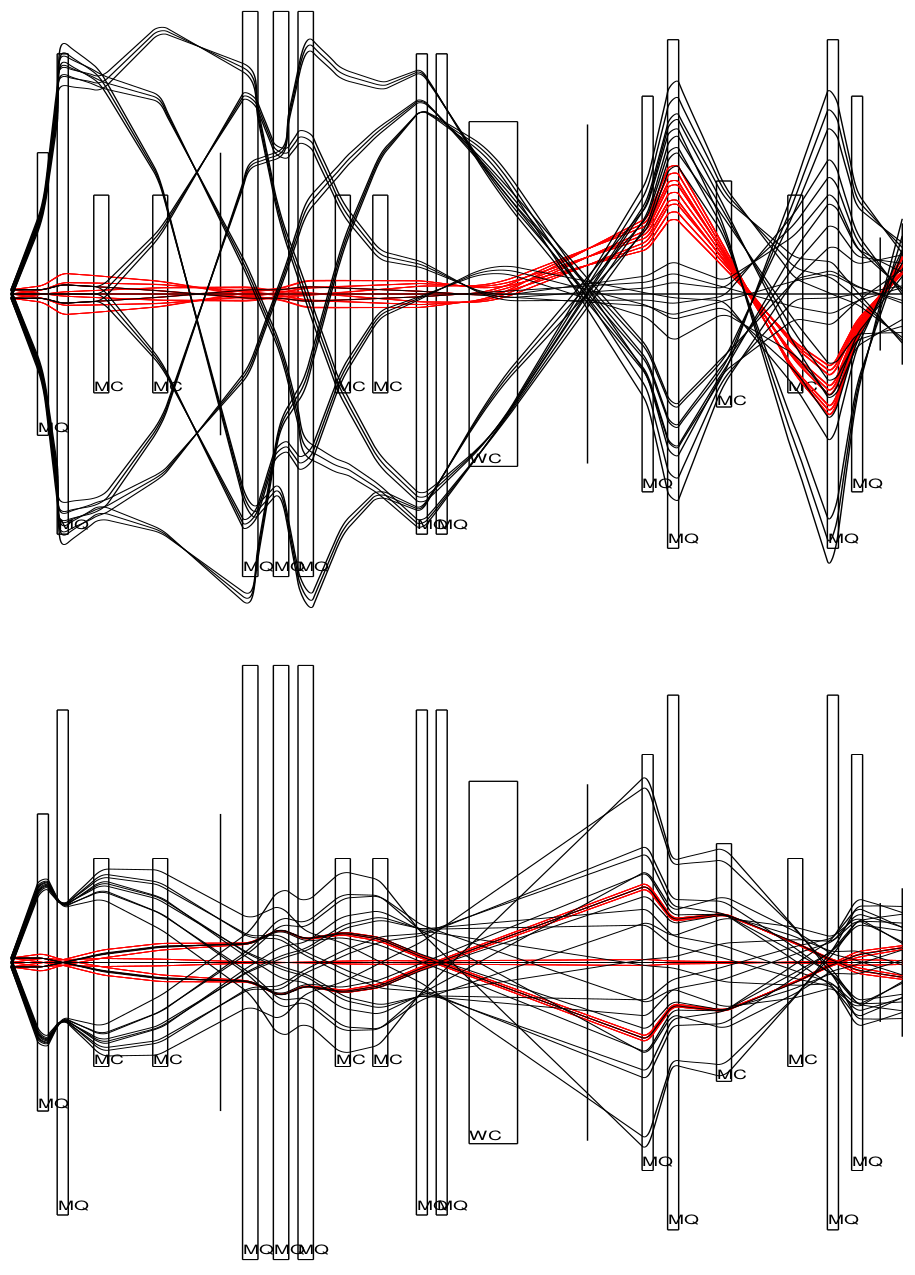
\includegraphics[width=0.8\textwidth]{figures/raytrace.png}}
        \caption[Horizontal and vertical rays through St.\ George]{Horizontal
            (upper plot) and vertical (lower plot) rays through St.\ George.
            Recoil \nuc{41}{Sc} rays are shown in black and beam \nuc{40}{Ca}
            rays are shown in red.
            % The beam energy is
            % $E_{\textrm{beam}} = 15.99\pm0.001$~MeV, and the recoil energy is
            % $E_{\textrm{recoil}} = 15.6\pm1.155$~MeV.
            The beam rigidities are $B\rho = 0.331$~Tm and $E\rho = 2.907$~MV,
            and the recoil rigidities are $B\rho = 0.331$~Tm and
            $E\rho = 2.836$~MV. Both the beam and recoil
            are taken to be in the $11^+$ charge state.
            The COSY calculation assumes that the recoil particles are spread
            within an acceptance range of $\Delta E/E \approx7.5$\,\% and
            $\Delta\theta = 40$~mrad. The transverse scale is highly
            exaggerated to show detail.}
        \label{fig:raytrace}
    \end{center}
\end{figure}


\section{Theoretical and Experimental Considerations}
\label{sec:cosy}

% Possibly move this to Chapter 2...

St.\ George was modeled within COSY Infinity (COSY-$\infty$, henceforth
\emph{COSY}), a beam optics and transport language developed at Michigan State
University~\cite{COSY}. The initial ion optics solution for the separator was
calculated by
Drs.\ Couder and Berg at the University of Notre Dame to maximize the angular
and energy acceptance for a point-like target located prior to the separator.
Optimization of the individual elements' properties allowed the separator
to achieve the previously-stated energy and angular acceptances, create an
achromatic focus at the mass slits (focal plane $F_2$), and transport all
recoils to the final detector focal plane $F_3$ (see Section~\ref{sec:stg}).
Each magnetic element is represented by a single command within the code,
defining the type and properties of the desired element. The three types of
elements used within St.\ George\----{}dipoles, quadrupoles, and the Wien
filter\----{}require different sets of values to be defined. The recoil
envelope, consisting of a number of sample recoil properties used as
representative rays, for the final designed configuration is shown in
Fig.~\ref{fig:raytrace}. For the example shown, the quadrupole pole tip fields
are given in
Table~\ref{tab:poletip}, where negative values represent a quadrupole focusing
in the $y$-direction. The pole tip fields for $(\alpha,\gamma)$ experiments are
for the test particles shown, while those for $(\rm{p},\gamma)$ experiments are
specific to this work (see Section~[REFERENCE]). The actual fields used will
depend on the rigidity of the desired particle to transport through the
separator and can be scaled from these values.

The initial ion optics solution creates a transport map for particles passing
through the entire separator that can be analyzed independently of the ray
traces and provide the mathematical backing to the particles' trajectories
within St.\ George. The transport map is dependent on the quantities
\begin{equation}
    \label{eq:cosyvars}
    \begin{split}
        r_1 &= x \\
        r_3 &= y \\
        r_5 &= l = -(t - t_0)v_0\gamma/(1 + \gamma) \\
        r_7 &= \delta_m = (m - m_0)/m_0
    \end{split}
    \quad\quad
    \begin{split}
        r_2 &= a = p_x/p_0 \\
        r_4 &= b = p_y/p_0 \\
        r_6 &= \delta_K = (K - K_0)/K_0\\
        r_8 &= \delta_z = (z - z_0)/z_0,
    \end{split}
\end{equation}
where $a$ and $b$ are analogous to angles within each plane, $\delta_K$ is the
energy difference from the desired energy $K_0$,
$\delta_m$ is the mass difference from the desired mass $m_0$, and
$\delta_z$ is the charge from the desired charge state $z_0$~\cite{COSY}.
The desired quantities are the values used to calculate the magnetic
(Eq.~\ref{eq:brho}) and electric (Eq.~\ref{eq:erho}) rigidity, and thus set the
fields of the elements within St.\ George,
of the particle to be transported through the entirety of the separator.
The time of flight difference $l$ is not considered in analyzing the separator.
The transport map contains terms up to fourth order.

The original ion optics calculation used default parameters to describe the
fringe fields of the optical elements. A change in the shape of the fringe
field can change the trajectory of the particles within the separator, as the
total field that the particle interacts with changes in magnitude. Since the
fringe fields used to find the ion optics solution and those created by the
actual magnetic elements within St.\ George may be different, the required
field strength may also be different. The pole tip fields for a given particle
rigidity, determined by the current setpoint for that magnetic, must be found
experimentally, or a new ion optics solution using fringe field
parameterizations that more accurately reflect those exhibited by the magnetic
elements must be found. The procedures for each of the three different types
of elements necessarily differ based on what diagnostic equipment is available.

% This problem really only affects the focusing quadrupoles within the separator.
% While the dipole magnets are set based on the rigidity of the desired particle,
% those magnetic settings can also be determined by observing the trajectory
% within the separator itself. As the overall desire of the dipole magnets is to
% transport the desired rigidity down the center of the separator, diagnostic
% equipment aligned with this central axis can be used to ensure that the beam is
% traveling along this centerline. In doing so, the experimentally correct field
% setting for the dipoles can be determined without too much effort.
The magnetic settings for the dipole magnets, determined by the rigidity of the
particles, can be determined by observing the trajectory of the particles within
the separator, where trajectories close to the central axis are desired. As this
trajectory can be directly observed using diagnostic equipment aligned with the
axis, it is relatively easy for the required values to be found within some
confidence interval around the theoretically desired value. Once these coarse
values are found, the final values which direct the particle beam along the
magnetic optical axis of the following quadrupoles can be determined by
minimizing the off-axis steering effects of the quadrupoles by adjusting the
dipoles' magnetic fields within a small window of values.

Setting the Wien filter can be done in a similar manner. The electric field
strength is determined from the analyzed energy of the particle, the known
charge state, and the desired bending radius of the filter. Thus, the electric
field strength can be set to an exact value, requiring the magnetic field to
be set to match the properties of the electric field. The strength of the
magnetic field is set such that the bending radii of the two fields are the
same and so that the particle beam continues along the magnetic optical axis in
the same manner as described previously with the standard dipoles. The
Wien filter was designed with magnetic yokes at the entrance and exit of the
filter to restrict the magnetic fringe field so that it matches the electric
fringe field created by the electrostatic plates, and those must be adjusted to
their proper positions before the magnetic field can be set.

The magnetic quadrupoles, due to the inability to directly observe the trajectory
of the focused particles within the separator at all possible angles and energies
concurrently to achieve the required acceptance properties of the separator,
require a similarly complicated and restrictive procedure to determine the
experimental settings that match the results of the beam optics calculations.
The full procedure is outlined in \ref{sec:tuning_stg}.


\section{Separator Properties}

The elements, power supplies, and supports were provided by Bruker Biospin and
installed in 200X. The separator design requirements for the strengths of the
optical elements were based on the maximum beam energy of the older KN
single-ended Van de Graff accelerator and the possible charge states produced
by its internal ion source. The 5U and ion source have similar properties to
this system. The power supplies for the magnets provide highly stable direct
currents for each magnet individually, with $dI/I \approx 10^{-4}$ for the
quadrupoles and $dI/I \approx 10^{-5}$ for the dipoles. The upper current limit
is different for each magnet. The separator uses a robust
water cooling system able to maintain the required $80\pm2$~\degree{}F magnet
temperature for the entire system. The system is able to maintain the
temperature even when all magnets are at their maximum currents for extended
periods of time.

The Wien filter electrode power supplies are set separately based on their
voltage, with voltage stability $dV/V \approx 10^{-5}$ in the range commonly
used for experiments. The upper limits for these power supplies are
$\pm110$~kV, with voltages below $\approx 70$~kV used during previous work. The
stability of the voltage is dependent on prior conditions within the vacuum
chamber, requiring conditioning of the plates before higher voltages can be
achieved. For voltages above $\approx 50$~kV, the plates were conditioned to
voltages at least 10~kV above the desired setpoint to provide a stable running
condition. For lower voltages, no conditioning is necessary unless the vacuum
chamber was recently vented (exposed to atmospheric pressure gases).

The properties (entrance and exit apertures, length, maximum field strength,
good field region, etc.) were determined within the ion optics solution to
transport the desired recoils, and built to match those specifications. The
entrance and exit pole faces for the dipoles were designed to provide higher
order corrections to the particle trajectory, since additional higher order
magnets could not used~\cite{Couder2008}. Additionally, the shape of the
Wien filter electrostatic plates were designed such that the electric and
magnetic fringe fields were closely matched.


\subsection{Magnetic Fringe Fields and Effective Field Lengths}

Detailed two-dimensional magnetic field maps for multiple excitations of each
magnet were provided by Bruker. The field maps allow a check on the good field
region for each magnet and provide a description of the fringe fields. Field
strengths at each location are measured in mT. The fringe fields for each
magnet, excitation, and measurement radial distance can be analyzed separately
if desired. From this data, the shape of the fringe field and the effective
field length of the magnetic elements can be determined. As these values are
essential to setting the necessary values for the quadrupoles, the analysis of
the field maps focused on these elements.

A single edge fringe field is described by the Enge function given by
\begin{equation}
    \label{eq:enge}
    E(z) \equiv \frac{1}{1 +
        \exp\left[\sum_{i=0}^{N-1}{a_i}(\frac{-z}{D})^{i}\right]},
\end{equation}
where $a_i$ are the desired expansion coefficients, $D$ is the aperture
diameter, and $z$ is the longitudinal distance~\cite{Baartman2007}. The
formulation above is used within COSY to describe user-defined fringe fields.
For a short magnet, which the St.\ George quadrupoles can be considered to be,
the entrance and exit fringe fields are not completely independent of each
other, since the fringe fields extend into the central region of the magnet.
Instead of fitting each fringe
field separately, we can instead fit the entirety of the magnetic field
profile using a combined ``short'' quadrupole function, in terms of the Enge
function, given by
\begin{equation}
    \label{eq:shortquad}
    k(z) = k_0\left[E(L/2 + z) + E(L/2 - z) - 1\right],
\end{equation}
where $k_0$ is a scaling parameter for the central field and $L$ is the
effective field length~\cite{Baartman2007}. This formulation assumes a
symmetric field profile, as both the entrance and exit fringe fields are
modeled with the same Enge function. The effective field length, defined as
\begin{equation}
    \label{eq:efl}
    L = \frac{1}{B_0}\int_{-\infty}^{\infty} B(z)\, \textrm{d}z,
\end{equation}
where $B_0$ is the field strength at the center of the magnet,
is the field length if the field were described with a pure ``hard edge'' or
Heavyside function at the entrance and exit, i.e.\ no fringe fields.

\begin{figure}[t]
    \begin{center}
        \centerline{
            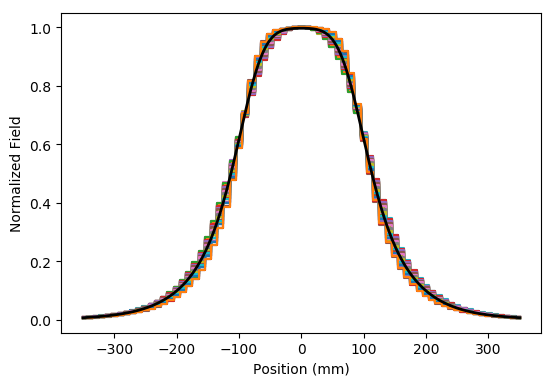
\includegraphics[width=0.85\textwidth]{figures/enge_fit.png}}
        \caption[Normalized field with Enge fit]{Normalized field and the
            resultant fit to the fringe field for the example quadrupole
            $Q_{10}$. The parameters of the fit are given in
            Table~\ref{tab:enge}.}
        \label{fig:enge_fit}
    \end{center}
\end{figure}

Using the field maps provided by Bruker, we can determine the Enge coefficients
and the effective field lengths for our magnets. For all calculations, since
the field near the center of the magnet is relatively weak, the fields within
2~cm in the radial direction of the central axis were not used for determining
either the effective field length or the Enge coefficients. Additionally, the
effective field length and the shape of the fringe field were assumed to not
differ with different magnet excitations, so all available data were used for
each magnet at the same time. An example using $Q_10$ of the normalized fields
used and the resulting fit is shown in Fig.~\ref{fig:enge_fit}.

The effective field lengths
were calculated directly from the field maps by integrating along the
$z$-direction for each radial distance provided. Since the maximum field
strength for a given magnet current varies depending on the distance from the
center, the individual ``traces'' of the magnetic field along the $z$-axis were
normalized. This normalization is shown in Eq.~\ref{eq:efl} as the constant
factor outside of the integral. The integration was performed using the
Simpson's Rule routine provided by the SciPy Python package~\cite{SciPy}. An
average of these lengths was used. Differences between the calculated effective
field length and those used within the initial ion optics solution were within
2\,\%. The new effective field lengths were used for all subsequent
calculations.

Using the same normalized field ``traces'' along the $z$-axis, the Enge
coefficients describing the shape of the fringe field may be determined. The
field profiles at each radial distance were fit simultaneously. Using the
default Enge coefficients as the initial parameter guesses, the summed mean
squared error between the data and Eq.~\ref{eq:shortquad} was minimized using
the Nelder-Mead downhill simplex minimization (see \cite{Simplex}) provided by
SciPy. The additional factor $k_0$ was included in the fit, but is not needed
when defining a fringe field within COSY. The process was repeated for each
quadrupole separately. The updated Enge coefficients and their comparison to
the default values used by COSY for $Q_{10}$ can be seen in Table~\ref{tab:enge},
and the difference in the shape of the fringe field can be seen in
Fig.~\ref{fig:enge_comparison}.

\begin{table}[t]
    \begin{center}
        \caption{ENGE COEFFICIENTS FOR $Q_{10}$ COMPARED TO COSY DEFAULTS}
        \label{tab:enge}
        \begin{tabular}{c S[table-format=2.8]S[table-format=2.6]}
            \toprule
            \midrule
            \textbf{Coefficient} & \textbf{$Q_{10}$ Values} &
                \textbf{COSY Defaults} \\
            \midrule
            $k_0$ &  0.99731489 & \\
            $a_0$ &  0.37255261 &  0.296471 \\
            $a_1$ &  6.18699778 &  4.533219 \\
            $a_2$ & -5.55514115 & -2.270982 \\
            $a_3$ &  6.96210851 &  1.068627 \\
            $a_4$ & -4.82581328 & -0.036391 \\
            $a_5$ &  1.3135787 &  0.022261 \\
            \bottomrule
        \end{tabular}
    \end{center}
\end{table}

\begin{figure}[t]
    \begin{center}
        \centerline{
            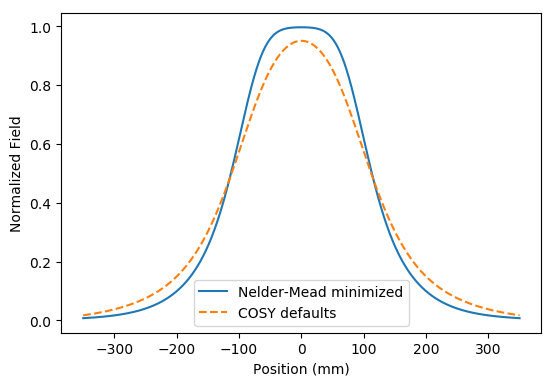
\includegraphics[width=0.85\textwidth]{figures/enge_comparison.png}}
        \caption[Comparison between fringe fields]{Comparison between fringe
            fields for the example quadrupole $Q_{10}$. The COSY default
            parameterization for the fringe field is the dashed orange line,
            and the fitted fringe field is the solid blue line. The distinct
            difference between the two field characterization requires the
            higher order effects arising from the fringe field to be taken into
            account.}
        \label{fig:enge_comparison}
    \end{center}
\end{figure}

In some cases, the field maps were not recorded far enough away from the center
of the magnet for the fitting routine to converge, primarily due to the field
not adequately reaching zero. In those cases, ``dummy'' points of zero field
were pre\---{} and post\---{}pended to the individual ``traces'' at distances
greater than 5~m from the center of the magnet to aide in convergence.

The default COSY coefficients for the fringe field were compared against the
data and shown to not adequately describe the field maps. The summed mean
squared error when using the short quadrupole formalization and the default
COSY parameters was significantly larger than that found through the
minimization routine, and the difference was shown to be statistically
significant. A visual comparison between the two models for $Q_{10}$ is shown
in Fig.~\ref{fig:enge_comparison}.


\section{Energy and Angular Acceptance}
\label{sec:commissioning}

The energy and angular acceptances of St.\ George were determined
experimentally through a series of experimental campaigns using multiple
rigidities. The energy acceptance without a corresponding angular acceptance
was shown to exceed the designed acceptance at zero degrees, with a measured
energy acceptance of $\Delta E/E = \pm 8$\,\% for ten different beam
rigidities covering the phase space region for astrophysically important
recoils~\cite{Meisel2017}. The angular acceptance has been shown to meet the
desired $\Delta\theta = \pm 40$~mrad in limited cases with an energy spread of
$\Delta E/E = \pm 3$\,\%. The full total acceptance has not yet been measured
within the designed phase space limits of St.\ George, with work ongoing.

Within the following discussion, the term ``test beam'' will be used in
reference to an incident beam produced by the 5U with a desired rigidity. These
test beams are defined by the beam particle, energy, and charge state selected
by the operator and produced by the 5U. These beams were chosen for to
provide particles with the desired rigidity and with beam currents in the range
of $0.5 - 3$~$\mu$A in order for the diagnostic equipment to properly measure
the beam. Additionally, those beams that commonly had highly stable 5U and ion
source running conditions over extended times were selected to reduce beam
preparation steps by the operators.

Acceptance measurements first probed the energy acceptance within the designed
$B\rho-E\rho$ phase space. The rigidity phase space
limits, along with measured acceptances and ranges for proposed future
experiments is shown in Figure~\ref{fig:rigidity_phase_space}. While it is not
possible to produce test beams with the 5U that completely span this phase
space, the regions of astrophysical interest are accessible, and work focused
on this region.

\begin{figure}[t]
   \begin{center}
       \centerline{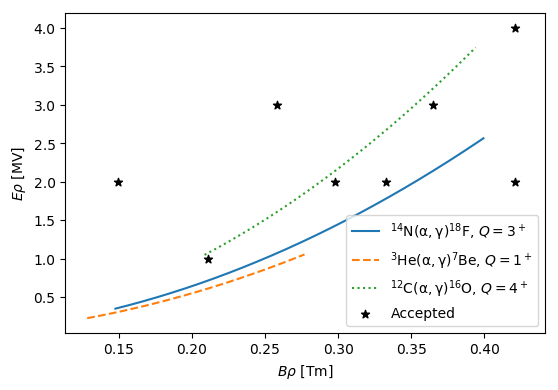
\includegraphics[width=0.8\textwidth]
           {figures/rigidity_phase_space.png}}
       \caption[Designed $B\rho-E\rho$ rigidity phase space for St.\ George]{
           Designed $B\rho-E\rho$ rigidity phase space for St.\ George. Stars
           represent rigidities that have been shown to have the full
           $\Delta E/E = 8$\,\% energy acceptance. Reactions shown are probable
           first experiments using St.\ George that use beam energies
           accessible with the 5U:
           \nuc{14}{N} at $E_{\rm{beam}}\approx 0.7-5.0$~MeV (solid blue line),
           \nuc{3}{He} at $E_{\rm{beam}}\approx 0.25-1.2$~MeV (dashed orange
           line), and
           \nuc{12}{C} at $E_{\rm{beam}}\approx 3.0-10.0$~MeV (dotted green
           line). These energy
           ranges cover some of the astrophysically important ranges for the
           given reactions.
           Adapted from~\cite{Meisel2017}.}
       \label{fig:rigidity_phase_space}
   \end{center}
\end{figure}


\subsection{Beam Tuning and Properties}
\label{sec:tuning}

The commissioning runs followed a similar procedure for beam preparation using
the 5U and the transport line. The beam rigidities were chosen to cover a
region within the phase space limits of the separator that cover recoils
produced through reactions of astrophysical interest. Both light (\nuc{1}{H}
and \nuc{4}{He}) and heavier (\nuc{16}{O} and \nuc{20}{Ne}) beams were used to
probe different regions of that phase space. Angular acceptance runs to date
have only used lighter beams. The energy uncertainty of the beam is
approximately 0.3~keV (see Section~\ref{sec:5U}), and a conservative value of
0.5~keV will be used when necessary.

Beam preparation can be divided into two segments: preparing the $\Delta E = 0$
test beam to enter into St.\ George along the central
magnetic optical axis, and transporting that beam along the central magnetic
optical axis within St.\ George. The following procedures were used for all
acceptance measurements, with differences being minor. The diagnostic equipment
described in Section~\ref{sec:diagnostic} was essential to performing the beam
preparation steps and their use is highlighted below.

\subsubsection{Before St.\ George}

The test beam must meet simple requirements in order to be useful for
commissioning St.\ George: it must enter St.\ George along the optical magnetic
axis, and it must have a narrow waist point with a circular cross section at
the target location. Additional requirements
were shown to be beneficial experimentally: the focus must not be highly
divergent, and the accelerator
must be providing highly stable beam current with low energy uncertainty. The
divergence of the beam was roughly known based on the focusing strength of the
preceding quadrupole magnets required to provide the desired beam properties
at the target location, with higher focusing strengths resulting in a more
divergent beam. A rough sketch of this relation is shown in
Figure~\ref{fig:divergence}.

\begin{figure}[t]
   \begin{center}
       \centerline{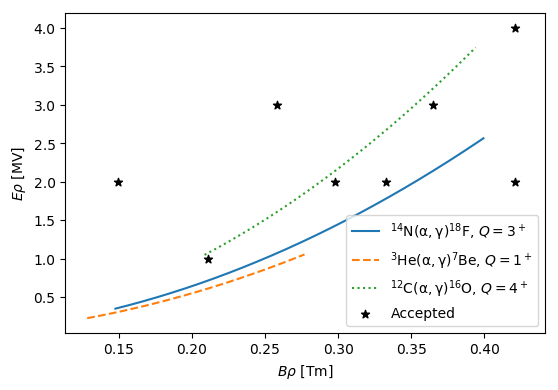
\includegraphics[width=0.8\textwidth]
           {figures/rigidity_phase_space.png}}
       \caption[Sketch of beam divergence due to focusing strength]{}
       \label{fig:divergence}
   \end{center}
\end{figure}

The beam intensity is dependent on which diagnostic equipment will primarily be
used. The isolated Faraday cups cannot read current below 50~$e$nA when read
through the logarithmic amplifier at the console,
and the current can't be above 20-30~$e\mu$A
as the cups are not currently water cooled and a high intensity and focused
beam may melt
some of the components. This upper current limit was not approached during the
tests, since the cups were used in tandem with the quartz viewers.
The quartz viewers are limited to
beam currents of a maximum of 3-5~$e\mu$A, as higher currents risk heating up
the quartz to
a high enough temperature to cause them to shatter or melt. Since four of the
quartzes
are also barriers between the high ($10^{-8}$~torr) vacuum within St.\ George
and atmosphere, this limit must be carefully avoided. In practice, currents
between 500~nA and 4~$\mu$A were used, based on the exact properties of the ion
source for that particular run, the beam species, and the locations of slits on
the primary transport line used to reduce the beam current.

The procedure for aligning the test beam to the magnetic optical axis is
described below. Major subsections of the procedure will begin with a short
title in bold to guide the reader. The elements on the main transport line that
may be necessary
to adjust are the switching magnet with the $X_6$ steerer, and the $Y_5$ and
$Y_6$ steerers (locations shown in Figure~[FIGURE]). The steerers are labeled
as such based on their position along
the main transport line. Steerers $X_6$ and $Y_6$ are part of the same physical
steerer but can be operated independently. Additionally, the quadrupole triplet
directly before the target location will be necessary for final tuning.

\textbf{Aligning the beam to St.\ George's optical axis:}
The desired test beam is transported down the St.\ George transport line and
monitored with the Faraday cup at the target location, called the
\emph{target cup} for beam current stability. Diagnostic equipment before the
target location are used as an aide to transport the beam and ensure that it
has the desired properties. If necessary, the beam current is reduced. The
quadrupole triplet is not be used at this point, since the beam may not be
entering the element along its magnetic optical axis.

The beam is sent into St.\ George. With no field in $Q_1$, $Q_2$, and $B_1$,
the beam hits the quartz viewer at the 0\degree{} exit port of the magnetic
vacuum chamber, called the \emph{$B_1$ quartz}. If the beam does not strike the
quartz, then the final set of steering elements needs to be adjusted to send
the beam into the quartz. When using the angular deflection commissioning
chamber, the current readbacks from the plates provides an additional
diagnostic on the trajectory of the beam.

\textbf{Checking for steering:}
Quadrupoles $Q_1$ and $Q_2$ are adjusted independently of each other, and the
resulting motion of the beam on the quartz is recorded. If the beam is aligned
with the central magnetic optical axis of either quartz, the quadrupole will
only focus the beam and not shift its position on the quartz, i.e.\ the spread
in the beam will
change but not its central position. The two quadrupoles must be adjusted
independently of each other as any induced steering from a beam misalignment in
one may be counteracted by a misalignment in the other quadrupole. If the beam
is steered by either quadrupole, the steering elements corresponding the the
focus direction of the offending quadrupole ($Y_5$ and $Y_6$ for $Q_1$, the
switching magnet and $X_6$ for $Q_2$) are adjusted to reduce the amount of
steering by that quadrupole.

A quadrupole steers a beam when the beam enters the magnetic element misaligned
with the optical magnetic axis. Assuming that the element is brought from zero
to defined strength, the focal length of the quadropule changes from
$\infty$ to a length $f$. The effect on the beam is that those regions of the
beam away from the optical axis are brought to pass through this focal point.
When a beam is aligned with the optical axis, there is an equal amount of the
beam on either side of this optical axis, so the beam spot will narrow along
the focusing axis of the quadrupole. The beam will also extend along the other
axis. If the beam is not aligned with the
optical axis, this beam motion to the focal point will be viewed as a lateral
motion along the focusing axis of the quadrupole.
A sketch of this effect can be seen in Figure~\ref{fig:steering}.

\begin{figure}[t]
   \begin{center}
       \centerline{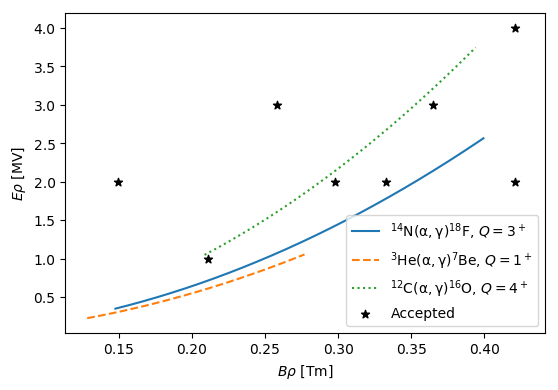
\includegraphics[width=0.8\textwidth]
           {figures/rigidity_phase_space.png}}
       \caption[Sketch of quadrupole steering of misaligned beam]{}
       \label{fig:steering}
   \end{center}
\end{figure}

The goal for adjusting the steering elements before St.\ George is to have each
quadrupole induce no steering on the beam. In practice, each change to the
steering elements either increases or decreases the amount of steering in the
direction of that element.
The crossover point, where the beam switches from steering left to steering
right for example, can be used to restrict the possible phase space of steerer
values, as the beam must have a zero deflection position between those two
extremes.

While each direction should be independent of each other, if the beam is far
from the magnetic optical axis, a single quad may induce steering in both
directions. When minimizing steering in a single direction, say the
$x$-direction, the other direction must also be checked frequently.

At the end of this process, the beam is not deflected when the field strength
for either $Q_1$ or $Q_2$ is increased or decreased independently of the other
quadrupole. The beam may be said to be entering St.\ George along the optical
magnetic axis. Due to the short distance between the first quadrupole doublet
and the $B_1$ quartz, it may be necessary to increase the sensitivity of the
steering to ensure that we are as aligned as possible to the axis.

\textbf{Increase sensitivity:}
The beam is then sent further into St.\ George, first to the $B_2$ quartz
located within the beamline then the $B_3$ quartz. The steering of $Q_1Q_2$ is
again checked in the same fashion as before. As these quartzes are located
further from the quadrupoles, they give a higher sensitivity to steering
affects from misalignment than just using the $B_1$ quartz at the trade-off
that the the quadrupoles can only be set to lower field strengths. Since the
quartz is further from the focusing elements, the same focusing strength will
create a larger beam spot on the quartz viewer. This effect can be seen in
Figure~\ref{fig:steering}.

These additional checks require $B_1B_2$ to have field. While these two dipoles
must have an exact field strength when performing acceptance measurements or an
experiment, at this point their fields only need to be coarsely set such that
the beam strikes the desired quartz. While the higher order corrections from
these magnets do play a role in the direction and focusing of the beam, that
contribution has no effect on determining beam alignment within the
quadrupoles.

The steering elements are adjusted in the same fashion to minimize steering in
$Q_1Q_2$. Since this steering was minimized during the previous step, these
adjustments should be minimal. It may
be necessary to have a weak field in $B_3$ in order to see the beam on the
$B_3$ quartz, due to possible machining misalignments of the port that the
quartz is attached to and the residual magnetic field within the dipole.

\textbf{Include the quadrupole triplet:}
As the last focusing element before St.\ George, the quadrupole triplet
(henceforth simply the \emph{triplet}) is the final adjustable element to
determine the beam properties when entering the separator. The triplet is used
to focus the beam to a small spot at the target location, a requirement for
both experiments and acceptance measurements. As it and $Q_1Q_2$ should lie on
the same magnetic optical axis, its steering must also be checked and minimized
if its use is desired for the present experiment. It was not used in all cases
as the coarse target focus provided by the previous quadrupole doublets on the
main transport line were deemed sufficient.

Before moving the beam off of the $B_1$ quartz, the steering effects of the
triplet must be characterized in the same fashion as $Q_1Q_2$. During the
steering minimization steps, both the triplet and $Q_1Q_2$ must both be
minimally steering before moving forward.

Due to minor misalignments between the triplet and $Q_1Q_2$, it is usually not
possible to have all elements nonsteering at the same time. In these cases, the
steering of $Q_1Q_2$ should take precedence while having the triplet minimally
steering. While the steering of the beam prior to the target location is
important, experimentally the steering of the individual elements within the
triplet cancel or nearly cancel each other out when the triplet is minimally
steering, reducing that problem.

At this point, the main transport line has been tuned to prepare a well-focused
and well-aligned beam entering into St.\ George. These elements are not to be
touched during the rest of the tuning process. The triplet, due to the
possibility of it having minor steering effects, must also have zero field for
the remainder of the steering checks, and will be turned on for the actual
measurement.

\subsubsection{Within St.\ George}
\label{sec:tuning_stg}

Once the test beam has been aligned to enter the separator along the magnetic
optical axis, it must also be aligned to the magnetic optical axes of all of
the quadrupoles within the separator. This alignment is done using only the
dipoles $B_{1-6}$ and the WF. Any minor misalignment in the vertical
direction should have been corrected during the previous steps, but there is
the possibility that there will be vertical steering within the separator, both
from that misalignment and effects from the dipoles and
quadrupoles. Within St.\ George, this equates to the $y$-focusing quadrupoles
($Q_{1,\,4,\,7,\,8,\,11}$) potentially steering minorly in the vertical
direction despite the best efforts of the operator. As there are no elements
within St.\ George that could correct for this, the steering effect of these
quadrupoles may not be able to be eliminated. The procedure for this second
alignment is straightforward, as the
only elements used to adjust the steering of the quadrupoles are the two
dipoles immediately prior.

\textbf{Tuning to the WF:}
With the beam striking the $B_3$ quartz, quadrupoles $Q_{3-5}$ are checked for
steering. The primary focus of these steering
checks will be on $Q_3$ and $Q_5$ which focus in the horizontal plane. The
magnetic fields within $B_1B_2$ are
adjusted to make these quadrupoles non-steering or minimally steering. The
field precision is on the order of 0.1~G, read back by the Hall probes.

Due to potentially small misalignments in the St.\ George quadrupoles in
relation to each other, it is commonly not possible to have $Q_{1-5}$
non-steering simultaneously (see \cite{Meisel2017}). In these cases, minimal
steering can be achieved through $Q_{3-5}$ when $Q_1Q_2$ are non-steering by
adjusting $B_1B_2$. At this point, dipoles $B_1B_2$ are set to the value
corresponding to the magnetic rigidity of the particle and to maintain the
test beam alignment to the optical axis.

Dipoles $B_3B_4$ are brought up to their rough field value to send the beam
through the WF and onto either the WF quartz or the $B_5$ quartz. The
quadrupoles $Q_{6-9}$ are checked for steering, adjusting $B_3B_4$ to minimize
the steering. Since there is some residual magnetic field within the Wien
filter, the electric field is brought up to compensate for this bending to keep
the test beam along the optical axis through $Q_8Q_9$. The field required is
calculated by determining the bending radius caused by the residual magnetic
field and creating the equivalent bending radius in the opposite direction for
the particle's $E\rho$.

As the beam envelope has expanded, it will be necessary to bring $Q_{1-5}$ to
their desired values in order to check the steering of the remaining
quadrupoles. Since these quadrupoles have been shown to be minimally steering,
their effect on the beam trajectory through remainder of St.\ George should be
negligible. It may be necessary to have a weak field in $B_5$ in order to see
the beam on the $B_5$ quartz for the same reasons as explained previously for
$B_3$.

\textbf{Setting the WF:}
For a test beam with $\Delta E = 0$ and $\Delta\theta = 0$, the elements within
St.\ George will be set to transport this along the central axis based on the
test beam's rigidity. Since the energy of the beam is well known and the charge
of the beam is exact, the electric rigidity $E\rho$ is also well known. The
electric dipole within the WF is set for this rigidity and held
constant for the remainder of the tuning process.

The magnetic field is set similarly to the other dipoles: to minimize the
steering induced by the next set of quadrupoles ($Q_8Q_9$). Since the test beam
was aligned to the optical magnetic axes of this quadrupole doublet in the
previous step, the WF magnetic dipole must return the beam to this
orientation. Additionally, since the elements within St.\ George act to
prepare the beam to be separated by mass by the WF, the quadrupoles
$Q_{1-7}$ must be set to the values determined by the test beam's magnetic
rigidity $B\rho$.

The magnetic field for the WF is read back using a Hall probe located
on the pole face. The field can be set precisely and related to the fields in
the other dipoles. Once the magnetic field is set such that $Q_8Q_9$ do not
steer the beam, the full WF is set.

\textbf{Tuning through the detector chamber:}
Dipoles $B_5B_6$ are set to their rough values based on the $B\rho$ of the test
beam, sending the beam through the detector chamber and onto the last quartz,
called the \emph{detector quartz}. As before, due to the size and shape of the
beam envelope, $Q_8Q_9$ must be set to the required values. The final two
quadrupoles $Q_{10}Q_{11}$ are checked for steering, and $B_5B_6$ are adjusted
to minimize that steering.

Since the test beam is traveling through the detector chamber, the entire
detection system must be pulled out of the way of the beam. Magnetic shields
have been placed below the MCP constructs to remove the effect of the magnetic
fringe fields on the beam deflection~\cite{MoralesDNP}. Once $Q_{10}Q_{11}$ are
non-steering, the test beam is fully aligned to the optical magnetic axis of
St.\ George.

\subsubsection{Collimator and Target Position}

The 2~mm diameter collimator at the target location
(see Section~\ref{sec:target}) is
used for setting the triplet to the proper values. A narrow waist beam at the
target location is a requirement to achieve the maximum angular and energy
acceptance
for St.\ George. With the collimator in place, the triplet is adjusted such
that the beam transmission, defined as the ratio between the beam currents
before and after the collimator as read by two separate Faraday cups, is
maximized and ideally close to 100\,\%.

Since the target chamber may rotate around its central axis, it is possible for
the location of the collimator to become slightly misaligned between runs.
Additionally,
the triplet may induce some minor steering at the target location, potentially
moving the focal point radially from the optical magnetic axis. The target
collimator position is then not a fixed value but must also be tuned to
maximize transmission. Once the collimator position is found, the target
position is immediately known.

Rotation angles between $-5$ and $+25$\degree{}, where 0\degree{} is to the
right from the beam's perspective, and extensions of $91-96$~mm of the mounted
linear motion have been explored. Maximum transmission has been found for
collimator positions within this range of rotation angles and extension
distances for multiple beams, restricting
the total possible search space for the collimator. Extensions of the
target ladder of $\approx 94$~mm, and rotation angles near $+10$\degree{} are
common ``best positions'' for the collimator.

For acceptance measurements, the collimator is used to create a focal point at
the target location. Once the beam preparation is complete, it is retracted
from the beamline. When a target is used as a degrader, the collimator position
is used to determine the target position.


\subsection{Energy Acceptance}

The energy acceptance of St.\ George at $\Delta\theta = 0$~mrad was measured to
be $\Delta E/e = \pm 8$\,\% for ten different rigidities (see
Fig.~\ref{fig:rigidity_phase_space} and \cite{Meisel2017}). The measurements
took place before the capability to measure the angular acceptance and will
be remeasured as part of a total acceptance measurement campaign. Test beam
rigidities were chosen to cover an adequate region within the designed phase
space near the rigidities expected for recoils of astrophysical interest and
based on the restrictions imposed by the 5U and ion source.

For a given set of field settings for a test beam at $\Delta E = 0$ that
provide 100\,\% transmission between the target cup and a Faraday cup located
within the detector chamber at focal plane $F_3$, the separator is said to
accept an energy difference if the test beam is changed to that different
energy and still have 100\,\% transmission between those two cups. To state that
St.\ George has an energy acceptance of $\Delta E/E = \pm 8$\,\%, a single set of
fields for the elements within the separator transmitted 100\,\% of the test beam
between the two cups when its energy was changed within that energy change.

The procedure for measuring the energy acceptance of a single rigidity is
outlined below. The slits located at the post-WF focal plane $F_2$
were used to define a beam center. As the tune for a given recoil is supposed
to be achromatic at this location, these slits were used as both a diagnostic
on the path of the beam and a check of this requirement during the
measurements. Note that the tuning process for these measurements did not make
use of the in-beam quartz viewers at $F_1$ and $F_2$ since they had not yet
been installed.

\textbf{Initial setup:}
After tuning a beam along the optical magnetic axis as described in
\ref{sec:tuning}, all elements within St.\ George are at a given field. The
dipole elements, including the WF, are not touched. The transmission
between the target cup and the $F_3$ cup is measured. If the transmission is
100\,\%, the beam energy was changed. If not, then the quadrupoles were retuned
to transmit 100\,\% of the test beam between the two cups.

Quadrupole retuning was done systematically to prevent over- or under-focusing
the beam at any location within St.\ George. With the beam on the $F_3$ cup,
each quadrupole was adjusted individually to determine what field is required
to transmit 100\,\% of the beam to the cup. After finding that field, the
difference is recorded and the quadrupole is returned to its original value.
This process is repeated for every quadrupole acting independently. If a single
quadrupole could not achieve 100\,\% transmission on its own, it was not included
in the next step. Assuming $N$ quadrupoles adjusted by $\Delta B_i$ to give
100\,\% transmission, the individual quadrupoles $Q_i$ were changed by
$\Delta B_i / N$. This approach usually resulted in achieving 100\,\%
transmission for the $\Delta E = 0$ case.

The quadrupole adjustment described was used at every step if the tune was
shown to not transmit 100\,\% of the test beam. Previous settings of the
quadrupoles were recorded to map regions of field strengths were 100\,\%
transmission was achieved for different energy changes.

\textbf{Changing energy:}
The beam energy was changed to $\Delta E/E = -8$\,\% by changing the accelerator.
The transport beamline was scaled automatically to account for the change in
rigidity. The beam was shown to enter into St.\ George along the optical
magnetic axis by putting the fields within $Q_1$, $Q_2$, and $B_1$ to zero and
checking the steering of the first two quadrupoles. Since this energy change is
minor, in most cases only the switching magnet needed to be changed. The
magnets $Q_1Q_2B_1$ were brought back to their required values and transmission
between the two cups was checked.

If the beam was fully transmitted to the $F_3$ cup, the settings for St.\
George were said to have an energy acceptance of $\Delta E/E = -8$\,\%. The beam
energy was then changed to $\Delta E/E = + 8$\,\%, following the same procedure,
and transmission was checked. If the beam also was fully transmitted, the
separator tune was said to have an energy acceptance of $\Delta E/E = \pm 8$\,\%
and the measurement was complete.

Where 100\,\% transmission was not achieved, the quadrupole scaling described
previously was used. The new tune was recorded, and the beam energy was
returned to $\Delta E = 0$ to check transmission. This process was continued
until all three energy points had 100\,\% transmission for a single setting of
St.\ George. During this cycling, referring to previous values was used to
prevent correcting the tune in one direction at one energy only to change back
to the previous tune at another energy.

Since the $F_2$ slits were placed around the beam center, achieving 100\,\%
transmission was only possible if test beam had a nearly or completely
achromatic focus following the WF, one of the requirements for normal
operation of the separator.

\textbf{Additional measurements:}
For subsequent energy acceptance measurements, instead of using the COSY
predicted values, an energy acceptance tune scaled based on the magnetic
rigidity $B\rho$ of the new test beam was used for the initial quadrupole
settings. If the difference in $B\rho$ was sufficiently small, the required
adjustments to the quadrupole fields were minimal, speeding up the measurement
process. As more individual energy acceptance measurements were made, the
scaling based on $B\rho$ became more robust to slight differences in beam
preparation and species.

Once the ten rigidities within the astrophysically interesting phase space of
the separator were measured, work moved to measuring the angular acceptance.


\subsection{Angular Acceptance}

As of this writing, the angular acceptance of St.\ George has been measured to
be $\Delta\theta = \pm 40$~mrad in the horizontal and vertical planes for a
single rigidity. The acceptance was shown by ensuring 100\,\% transmission
when deflecting the beam 40~mrad in each direction, and quadrupole adjustments
followed the same procedure as during the energy acceptance measurements. The
measurement was done without a corresponding energy acceptance, and without the
requirement that the test beam be focused at the focal plane $F_2$ following
the WF and without the beam passing through the slit opening at that
location for all deflection angles. The measurement was then a single ``proof
of concept'' that an angular acceptance could be measured using the new
diagnostic and control equipment installed. Due to complications with the
measurement process, multiple attempts at measuring the angular acceptance,
each with a different procedure, were tried. These attempts are outlined below.

\textbf{Deflector plates only:}
A test beam is tuned to provide a non-steering beam with 100\,\% transmission
between the target and $F_3$ cups. The deflector plates (see
Section~\ref{sec:target}) are rotated so that they deflect the beam in a single
plane. The horizontal plane was commonly chosen first. Since the entrance
aperture for the target cup is larger than 40~mrad, it does not intercept any
of the beam when it is deflected. Angles between 0 and 40~mrad were used and
the current on the $F_3$ cup was monitored. The maximum angle that provided
100\,\% transmission was recorded.

If the maximum angle achieved was not 40~mrad, the quadrupoles were tuned in
the same fashion as for the energy acceptance measurement but with the
deflector plate set to an angle greater than was accepted such that the beam
is still partially captured by the cup. The changes to the quadrupole fields
were recorded, and all quadrupoles that could provide 100\,\% transmission were
scaled to new values. The beam was returned to $\Delta\theta = 0$ to ensure
that the new tune still provided 100\,\% transmission in this case, and the
deflection was changed.

A single plane was checked for $\pm 40$~mrad first before switching to the
other plane, and any retuning was done to also transmit 100\,\% of the beam to
the final cup. The deflector was also rotated to check the other plane, and
the quadrupoles retuned to provide 100\,\%. In general, this procedure did not
provide 100\,\% transmission when deflecting a test beam up to 40~mrad in the
four cardinal directions. This procedure was used for the single full angular
acceptance measurement.

Additionally, since the angular and energy acceptance is dependent on the
beam extent and shape at focal plane $F_2$, the WF quartz was used to
aide in tuning $Q_{1-7}$ to their proper values. The beam should move minimally
at this location when deflected up the the maximum 40~mrad in any direction.
The beam profile is required to be horizontally narrow for the highest mass
separation, requiring the vertical extent to be large. Using this intermediate
quartz slightly improved the ability to tune the separator but did not allow
for a full angular acceptance measurement to be performed.

\textbf{Degrader foil:}
The limiting factor in using the deflector plates as the only angular change is
that each direction must be looked at independently. Assuming the plates are
aligned to deflect in the horizontal direction, only one direction (left or
right from the beam's perspective) can be viewed at a time without some
manual adjustment to the deflector plate power supply. The cyclic problem of
correcting the beam trajectory only to remove that correction becomes harder to
avoid. Since the plates can only deflect along a single plane, the additional
unknowns of removing a large angular acceptance along a difference by making
changes on the current plane also decreased the possibility of success.

At the target location, Al foils of different thicknesses were placed to
degrade the beam, creating a spread in angle and energy at the same time. Foil
thicknesses were matched with beam properties to fall within the anticipated
$\Delta E/E = \pm 8$\,\% and $\Delta\theta = \pm 40$~mrad acceptances of St.\
George. Since the foils also induce an energy loss for the test beam, the
separator dipoles needed to be properly scaled down to the correct values after
the test beam (without foil in place) was aligned to the magnetic optical axis.
The scaling required accurate and precise measurements of the foil thicknesses.
Thicknesses ranged from $100-250$~$\mu$g/cm$^2$, and \nuc{1}{H} and \nuc{4}{He}
test beams in the energy range of $0.9-2.0$~MeV were used.

Using the WF quartz, the test beam was tuned to have the correct phase space
properties at $F_2$. The degraded test beam is emitted into the separator
within a phase space determined by its interaction with the foil, allowing the
magnets to be tuned without relying on the slow change between deflection
angles and directions and including the minor energy acceptance measurement.
Currently, no full angular acceptance measurements have been made past $F_2$.

% Dalmore 12 Year - The Exchange

\textbf{Reaction Measurement:}
Additional measurements have been made of the angular acceptance with an
energy acceptance and a nearly achromatic focus at the $F_2$ focal plane. These
measurements were for the altered settings for transporting $\alpha$ particles
from $(\textrm{p},\alpha)$ reactions. The measurements are a different ``proof
of concept'' for the angular acceptance measurements by verifying a
$\Delta\theta = \pm 40$~mrad acceptance with the deflector plates before using
a foil to produce the full angular spread. In this case (see [SECTION]), the
transported particles are the reaction product $\alpha$ particles, verified
using a direct test beam of $\mnuc{4}{He}^{2+}$. The transported reactions
products within the $\approx 45$~mrad cone limited by the target Faraday cup were
transported to $F_2$ and detected with the Si detector.


\section{Considerations}

Full acceptance measurements require a fine detailed understanding of the
operation of St.\ George. Previous work has provided the initial understanding
on providing a large energy acceptance of at least $\Delta E/E = \pm 8$\,\% and
angular acceptances near $\Delta\theta = \pm 40$~mrad. Combined measurements
have been limited to a large energy acceptance and small angular acceptance or
vice versa. Current work is ongoing on providing an improved understanding of
the operation of St.\ George, particularly in setting the quadrupole fields.

A full commissioning of the separator system requires the gas target,
separator, and detection system to be operated in parallel and well-understood.
The current status of each of these discrete systems is varied. The Hippo gas
target has been tested in a prior configuration, and work has been started to
redesign the upper chamber to improve the possibility for monitoring incident
beam current and using a $\gamma$ detector in coincidence with the final
detector system. The combined $E_{\rm{TOTAL}} vs. TOF$ detection system has
been shown to work for test surface sources. Silicon detectors are known to be
very robust, and the Si detector and acquisition system has been used for
a successful measurement with St.\ George for $(\rm{p},\alpha)$ measurements.
The separator status has been explored earlier in this chapter. Final
verification of the separator will be measuring the test reaction
\react{\mnuc{14}{N}}{\alpha}{\gamma}{\mnuc{18}{F}} in inverse kinematics.

The target chamber used for the commissioning work and the experimental
campaign is different than that which will be used during a fully featured St.\
George experimental campaign, namely the Hippo supersonic helium gas jet
target. Hippo will be used for $(\alpha,\gamma)$ experiments following the
completion of the commissioning work. The specifics of that gas target are
discussed elsewhere (see \cite{Kontos2012} and \cite{Meisel2016}). Due to the
differences between the commissioning chamber and the design of the gas target,
some specifics of beam tuning and preparation (see Sec.~\ref{sec:tuning}) will
inevitably change as experimental work transitions between commissioning and
reaction research work.

\chapter{MEASURING THE \alpa{} CROSS SECTION}

% \begin{center}\textit{Alphas have more mass because they spend so much
% time at the gym getting swole. \---{} Laura Moran}\end{center}

An experimental campaign to study the \alpa{} reaction with the St.\ George
recoil separator was undertaken at the NSL. Runs were completed in December
2016 and February 2017, with runs focusing on determining the correct magnetic
fields within St.\ George completed in Fall 2016 and February 2017. Two low
energy resonances were measured with beam currents in the $2-3$~$\mu$A range in
February 2017. Studying this reaction provides a test of the angular and energy
acceptances of St.\ George in preparation for studying $(\alpha,\gamma)$
reactions across a wide range of targets and energies.

The first portion of these runs fall under general St.\ George
commissioning work as discussed in Chapter~\ref{ch:commissioning} and will not
be repeated here. The second portion of the runs involved characterizing the
target and the detector, finalizing the optimal settings for the separator, and
performing the experiment. The reaction of interest produces $\alpha$ particles
in the energy range of $2-3$~MeV for the desired proton energy range.


\section{Altered Tune}

The magnet settings for St.\ George were determined to transport $\alpha$
particles, where the entirety of the particle envelope is described by a
characteristic energy and angular [term]. The produced $\alpha$ particles had
a low (values?) energy spread and a high angular spread, where only those
particles emitted within the desired 40~mrad acceptance cone for St.\ George
were tuned to reach the detector focal plane $F_2$ after the Wien filter and
impinge the installed Si strip detector.

The restrictions on the beam spot for measuring $(\rm{p}\alpha)$ reactions
at this focal plane require an approximately symmetric spot size in both
directions and one that
is smaller than the physical face of the detector, whereas the standard tune
for studying $(\alpha,\gamma)$ reactions required that beam spot to be
asymmetric with the beam spot being narrow in the dispersive $x$-plane and
tall in the $y$-plane. The initial COSY code for St.\ George
(see Section~\ref{sec:cosy}) was altered
to model the shortened separator and provide information on the beam
characteristics at the new detector focal plane. The magnetic field settings
for the seven quadrupoles $Q_{1-7}$ were adjusted to transport the recoil
particles to the detector plane with a final beam spot no larger than the face
of the Si detector of $58\times 58$~mm. Final pole tip fields are given in
Table~\ref{tab:poletip}.

\begin{table}
    \begin{center}
        \caption{POLE TIP FIELDS FOR $(\alpha,\gamma)$ AND
            $(\rm{p},\alpha)$ STUDIES}
        \label{tab:poletip}
        \begin{tabular}{cS[table-format=2.9]S[table-format=2.6]}
            \toprule
            \midrule
             & \multicolumn{2}{c}{\textbf{Pole Tip Field [T]}} \\
            \textbf{Quadrupole} & {$(\alpha,\gamma)$} & {$(\rm{p},\alpha)$} \\
            \midrule
            1  & -0.16303276 & -0.157\\
            2  &  0.18882363 &  0.187\\
            3  &  0.09384148 &  0.09411\\
            4  & -0.12620402 & -0.04\\
            5  &  0.10032405 &  0.092 \\
            6  &  0.04693654 &  0.0585 \\
            7  &  0.0        & -0.015 \\
            8  & -0.09779179 & \\
            9  &  0.17439627 & \\
            10 &  0.21092228 & \\
            11 & -0.13962355 & \\
            \bottomrule
        \end{tabular}
    \end{center}
\end{table}

For the $(\rm{p},\alpha)$ experiment, the transported $\alpha$ particles
have the properties listed in Table~\ref{tab:alpha_prop}. The incident proton
beam is rejected within the COSY ion optics solution after the first dipole
doublet $B_1B_2$, and the beam properties are not listed here.

\begin{table}
    \begin{center}
        \caption{ALPHA PARTICLE PROPERTIES}
        \label{tab:alpha_prop}
        \begin{tabular}{cc}
            \toprule
            \midrule
            \textbf{Property [Unit]} & \textbf{Value} \\
            \midrule
            Energy [MeV]        & 2.504 \\
            $\Delta$Energy [\%] & 3 \\
            Angular spread [mrad] & 40 \\
            Target diameter [mm] & 3 \\
            $Q$ [$e$]           & 2 \\
            $B\rho$ [Tm]        & 0.228 \\
            $E\rho$ [MV]        & 4.0 \\
            \bottomrule
        \end{tabular}
    \end{center}
\end{table}



\section{Experimental Considerations}

\subsection{Beam Reduction}
Incident proton beam reduction on the order of $10^{10} - 10^{14}$ are required
to avoid damaging the Si detector and observing off-resonance yields of the
produced $\alpha$ particles. These limits are within the designed capabilities
of St.\ George but must be verified experimentally

% Glenlivet 12 Year



\section{Procedure}

The procedure for performing the \alpa{} measurements is divided between the
experimental procedure and the procedure to measure a single energy point for
clarity. Verification of the initial field settings of St.\ George was
discussed in Section~[REFERENCE] as is assumed for the remainder of this
discussion.

\subsection{Campaign Procedure}



\subsection{Run Procedure}

At each energy point, preliminary runs were performed to verify the field
settings of St.\ George and determine the systematic uncertainties of the tune.
Following these checks, a final measurement at that energy was performed until
the statistical uncertainty was below 1\,\% for on-resonance points and below
5\,\% for off-resonance points.




\section{Data Reduction and Analysis}

Each region of interest covered a single narrow resonance from the \alpa{}
reaction. Extraction of resonance parameters from these regions required a
data analysis pipeline to process the individual spectra from each strip of
the Si detector and the detector spectra as a whole. Detection systematic
uncertainties were determined individually for each energy measure prior to
the final measurement at that energy. Target effects on the incident beam
and produced $\alpha$ particles were explored [HOW?].

\subsection{Experimental Systematics}
The properties of the target, detector, and separator for the given experiment
were explored through various means before, during, and after the data
collection phase. Where applicable, the properties were compared to anticipated
or predicted values. Differences between operating and testing conditions may
be a cause of certain discrepancies within the detector spectra, as discussed
below.

\subsubsection{Target Properties}
The self-supporting \nuc{27}{Al} target was measured to have a thickness of
$62.50 \pm 0.05$~$\mu$g/cm$^2$. Target thickness was measured using an offline
detector station with a \nuc{241}{Am}/\nuc{148}{Gd} mixed $\alpha$ source. Runs
with and without the target foil between the source and the detector lasted
600~s. The annular Si detector was not able to resolve the lowest intensity
\nuc{241}{Am} peak during the runs, and only the highest intensity peak could
be reliably resolved in the spectrum obtained with the target in place. The two
spectra are shown in Fig.~\ref{fig:calibration}, and the $\alpha$-particle
peaks are given in Table~\ref{tab:calibration}.

\begin{figure}[t]
    \begin{center}
        \centerline{\includegraphics[width=1.0\textwidth]%
            {figures/target_thickness.png}}
        \caption[Target thickness measurement]{Target thickness measurement,
            showing the shift in the $\alpha$ peaks to lower energies due to
            the presence of the target. The initial spectrum is in green and
            the degraded spectrum is in orange. Only the energy range of
            interest is shown.}
        \label{fig:calibration}
    \end{center}
\end{figure}

\begin{table}
    \begin{center}
        \caption{ALPHA PARTICLE ENERGIES FOR \nuc{241}{Am}/\nuc{148}{Gd} MIXED
            SOURCE}
        \label{tab:calibration}
        \begin{tabular}{cS[table-format=5.3]%
                S[table-format=3.1, table-space-text-post=\,\%]}
            \toprule
            \midrule
            {\textbf{Isotope}} & {$\mathbf{E_{\alpha}}$\textbf{ [keV]}} &
                {\textbf{Intensity}} \\
            \midrule
            \nuc{148}{Gd} & 3182.69 & 100\,\% \\
            \nuc{241}{Am} & 5388    &   1.6\,\% \\
                          & 5442.8  &  13.1\,\% \\
                          & 5485.56 &  84.8\,\% \\
            \bottomrule
        \end{tabular}
    \end{center}
\end{table}

The spectra were calibrated from the source-only run using the known energies
of the emitted peaks. The shift in energy of the two largest peaks were
recorded. The expected range for each peak was determined by interpolating the
tabulated results from SRIM~\cite{SRIM}. The target thickness was the difference in
range for each peak between the degraded and undegraded $\alpha$ energies.

During the experiment, the total time of beam on target was minimized to limit
the amount of carbon deposited on the target. Total charge accumulation on the
order of 100~mC, with $\approx 75$~mC from the final measurement runs. The
longest measurement run deposited $\approx 25$~mC on the target. At
these levels, no appreciable change to the target thickness during the
experiment could be seen. The target thickness was not remeasured following
the end of the experimental campaign.


\subsubsection{Detector Properties}
The 16-strip Si detector was caibrated using a \nuc{241}{Am}/\nuc{148}{Gd}
mixed $\alpha$ source. Calibration runs were taken before and after the data
collection phase, since the bias voltage was changed for the final runs. The
final calibration run was taken with the same electronics setup and detector
installation as during the run, except that the beam shield was removed.

Each strip and ADC were calibrated separately. A linear fit was used, as there
only the two highest intensity $\alpha$-particle peaks were resolved. Bins
were shown to be approximately 2~keV for every strip. The resolution is cited
for only the $E_{\alpha} = 3182.69$~keV peak from \nuc{148}{Gd} as this is
closer in energy to our expected particles. The calibration constants and
detector resolutions are shown in Table~\ref{tab:calibration_results}.

The efficiencies of the individual strips were not determined and assumed to be
100\,\% for all. Measurements of similar detectors for the St.\ George detector
system commissioning work showed $>99$\,\% efficiencies across all strips.

The detector response shows low energy tails for both alpha peaks (see
Fig.~\ref{fig:response}). The data show that the $\alpha$ events may fall
outside of the two peaks. All events within our detector can then be considered
real events, reducing the reliance on the energy calibration. The data also
shows that the lower intensity \nuc{241}{Am} $\alpha$ peaks cannot be resolved.

\begin{table}
    \begin{center}
        \caption{DETECTOR ENERGY CALIBRATION AND RESOLUTION}
        \label{tab:calibration_results}
        \begin{tabular}{cS[table-format=4.2]S[table-format=1.4]%
                S[table-format=1.2, table-space-text-post=\,\%]}
            \toprule
            \midrule
            {\textbf{Strip}} & {$\mathbf{a_0}$\textbf{ [keV]}} &
                {$\mathbf{a_1}$\textbf{ [keV/ch]}} & {\textbf{Resolution}} \\
            \midrule
             1 &  -85.61 & 1.6534 & 1.92\,\% \\
             2 & -165.12 & 1.7327 & 2.67\,\% \\
             3 & -123.66 & 1.5791 & 2.38\,\% \\
             4 & -172.41 & 1.6824 & 2.71\,\% \\
             5 & -194.53 & 1.6923 & 2.71\,\% \\
             6 & -235.36 & 1.7636 & 2.88\,\% \\
             7 & -202.59 & 1.7946 & 2.99\,\% \\
             8 & -203.93 & 1.8526 & 2.85\,\% \\
             9 & -269.19 & 1.8725 & 3.00\,\% \\
            10 & -252.46 & 1.8166 & 3.03\,\% \\
            11 & -243.02 & 1.8509 & 2.91\,\% \\
            12 & -272.25 & 1.8291 & 2.87\,\% \\
            13 & -235.06 & 1.8161 & 2.97\,\% \\
            14 & -172.81 & 1.7601 & 2.77\,\% \\
            15 & -235.26 & 1.8246 & 3.10\,\% \\
            16 & -110.00 & 1.6412 & 2.17\,\% \\
            \bottomrule
        \end{tabular}
    \end{center}
\end{table}

\begin{figure}
    \begin{center}
        \centerline{\includegraphics[width=1.0\textwidth]%
            {figures/calibration_overlay.png}}
        \caption[Detector response example]{Example of the detector response
            from the energy calibration run. All 16 calibrated strips are
            overlayed to better show the overall trend. Long, low-energy tails
            from both calibration peaks can be seen. The counts in the lowest
            energy range are noise.}
        \label{fig:response}
    \end{center}
\end{figure}


\subsubsection{Separator Properties}
The energy resolving power is the minimum energy difference required to resolve
a peak from the central image peak assuming that the change in energy is the
only difference between the two peaks. By definition this quantity is only a
first-order value, so only those parameters with a linear relationship with the
position need be considered. The energy resolving power of the separator
in relation to the terms present in the COSY transport map is defined as
\begin{equation}
    \delta_k(\textrm{RP}) \equiv
        \frac{2\left[(x|x)x_0 + (x|a)a_0\right]}{(x|\delta_k)},
\end{equation}
where $x_0$ and $a_0$ are the initial half-widths for position (in meters) and
angle (in radians), respectively, and the remaining terms are the values from
the transport map. The resolving power is only taken in the horizontal plane
due to the vertical symmetry of the separator. The terms taken from the
transport map are
\begin{align*}
    (x|x) &= 2.261610 \\
    (x|a) &= {-0.1368242} \\
    (x|\delta_k) &= {-0.2774295},
\end{align*}
where signs are conserved for completeness. The maximal deviation caused by
each terms is taken to be a positive value. The half-widths $x_0$ and $a_0$ are
physically limited by the target chamber and taken to be $x_0 = 1.5$~mm and
$a_0 = 42$~mrad, giving a resolving power of $\delta_k(\textrm{RP}) = 0.286$.
Since the produced $\alpha$ particles have an inherent spread in energy due to
the incoming beam and the particles themselves interacting with the target, the
energy resolution should be viewed as the window within which the energies are
indistinguishable. As this window covers the expected energy spread of the
produced $\alpha$ particles, there are no energy corrections required across
the detector strips.


\subsection{Yield Extraction}
For each energy, the number of $\alpha$-particle ejectiles produced was the
total sum of counts within each detector strip above the maximum proton energy.
Due to the detector response, any event above the noise threshold at
$\approx 200$~keV is a potential $\alpha$ event. There is still the possibility
that some of the incident proton beam strikes the detector despite the
rejection capabilities of St.\ George, so those counts below the maximum proton
energy are rejected. The maximum proton energy is taken as the incident beam
energy plus 3\,\% to be conservative. Since the proton beam is degraded in
energy based on its interaction with the thin foil, this upper limit for the
proton energy and lower limit for the $\alpha$ energy range will prevent any
proton-induced counts from being counted. An example is shown in
Fig.~\ref{fig:proton_peak}. While most runs did not show a discernible peak at
the expected energy, this cut was still made. In those cases, ``lost'' counts
were smaller than the statistical uncertainty of the counts above the energy
threshold.

\begin{figure}[t]
    \begin{center}
        \centerline{\includegraphics[width=0.85\textwidth]%
            {figures/proton_peak.png}}
        \caption[Possible proton peak]{Possible proton peak within the spectrum
            of a single ADC. Data is from Run 241
            ($E_{\textrm{p}} = 1.1781$~MeV). The vertical dashed line shows the
            energy cut, with the potential beam peak below this energy. The
            remaining 15 strips for this run showed a similar peak in both
            central energy and counts.}
        \label{fig:proton_peak}
    \end{center}
\end{figure}

Beam currents at the target location were recorded before and after each run.
For runs lasting longer than 15~m, the current was recorded every 15~m. The
beam current was seen to fluctuate around the recorded value by up to 100~nA.
For runs with multiple current readings, the average was taken as the nominal
current. Time on target was recorded by the acquisition system.

The total yield for each energy is given by $Y(E) = N_r / N_b$, where $N_r$ is
the number of reaction products produced and $N_b$ is the number of incident
beam particles. If we include the detector and transport efficiency of our
setup, and relate $N_b$ to our incident beam current, our yield becomes
\begin{equation}
    \label{eq:yield}
    Y(E) = \frac{N_r}{\epsilon_d\epsilon_tI_bt}.
\end{equation}
In this case, we assume that the detector and transport efficiencies are
100\,\%, based on the usage of a Si detector and the setting of St.\ George
to create a 100\,\% transmission state.

The uncertainties in the number of incident beam particles come from the
uncertainty in the collection time at the detector and the uncertainty or
walk within the incident beam current arriving at the target location.
Due to the start-up and shut-down timing for the DAQ, a time uncertainty of
5~s was adopted for each run, which should be a conservative value.
Without the offset Si detector to measure scattering at the target, we
do not have a direct measure of the beam current \textit{in situ} and must
rely on the beam currents measured before and after a given experimental run.
From those measurements, and from previous experimental runs using the 5U,
an uncertainty of 0.1~$\mu$A (less than 5\,\% in most cases) was adopted.
Final uncertainty for the number of incident particles is thus below a 5\,\%
statistical threshold.

% systematic for beam current stability...?

The uncertainty in the number of reaction products produced can be divided
between the statistical uncertainty in the counting of particles at the
detector and the systematic uncertainty of the missed particles at the
detector plane due to the tuning of the magnetic and electrostatic elements
of St.\ George. The statistical uncertainty of the counts is $\approx 5$\,\%,
as experimental runs were continued until this point. The systematic uncertainty
can be approximated by using the additional runs performed before the actual
experimental run, used to finalize the tune of the Wien filter and to estimate
the loss below the detector position, to estimate the ``lost'' counts
arising from the final experimental configuration of the separator.

% determine systematic uncertainty


The mounted target is a $62.50\pm0.05$~$\mu$g/cm$^2$ self-supporting Al foil
provided by Dr.\ Simon's group at the NSL. The target thickness was determined
with a mixed \nuc{241}{Am}/\nuc{148}{Gd} $\alpha$ source, providing $\alpha$
particles across the expected energy range, as shown in Table~[REFERENCE].
Only the two highest intensity peaks in \nuc{241}{Am} could be reliably
discriminated from the background, thus providing only three energy points for
calibration purposes of the detector. Target thicknesses were measured using an
offline setup, consisting of a Si detector within a vacuum chamber connected to
a data acquisition system. Data was recorded using MAESTRO for Windows
[REFERENCE] and converted using \texttt{pyne}.




\section{Detector Spectrum
Verification}\label{detector-spectrum-verification}

Due to the suboptimal energy resolution of the Si strip detector, caused
by the decreased bias voltage and increased leakage current, a
well-defined spectrum for the produced $\alpha$ particles was not
obtained. The spectra for each run and each strip show a wide peak at
the expected location of the $\alpha$ energy peak which we need to
verify that it represents the same underlying expected energy peak
produced in the reaction. This final verification is a convolution of
the incident beam energy, the properties of the target, the cross
section domain that we are probing, and the energy resolution of the
detector. Each of these components will be discussed in turn.

To reduce this check to a smaller subset of possibilities, only the two
resonance energy runs will be checked, but the same process described
below can be repeated for any energy in question, given the existence of
the required files to support the analysis.

This analysis relies on the usage of SRIM/TRIM [CITE] to generate
the files describing the target effects, and those files should be
generated according to the steps described below before the analysis is
begun. The file generation can be done programmatically following the
SRIM user guide, or ``by hand'' using the included GUI, both of which
are standard procedures and will not be discussed here.


\subsection{Assumptions}\label{assumptions}

In order to fully describe reaction process from incident beam to
detector energy spectrum, we must make some assumptions and check that
they are approximately true for the desired reaction.

First, the stopping power of the target must be slowly varying across
the width of the target. This assumption reduces the number of required
SRIM files, as described below. The definition of ``slowly varying'' in
this case is that the stopping power can be locally modeled as a linear
function of the beam energy, and that the coefficient relating the
energy to the stopping power be relatively small.

Second, knowledge of the underlying cross section is required. The
procudure described below can be inverted slightly to move from the
detector energy spectrum to the reaction cross section, knowing all
other parts, but this more-complex procedure was not required for the
reaction in question. Using known resonance properties, the
\react{\mnuc{27}{Al}}{rm{p}}{alpha}{} reaction cross section
can be modeled with the AZURE [CITE] $R$-Matrix code to produce
the file. The energies returned from this code should be transformed
into lab coordinates.

Third, the target should be thin enough that the beam can pass through
the target relatively unimpeded. Should this assumption not be met, the
procedure outlined must be updated to account for the additional
straggling, especially where the exit angle of the particles is
sufficiently spread out.

Finally, the thickness of the target in energy for the incident beam
energies must be known. Given that the thickness in
$mu\rm{g}/\rm{cm}^2$ can be measured using standard techniques,
the thickness in energy can be determined by
\[
    EQUATION HERE,
\]
where $d\rm{E}/dx$ is the stopping power in units of [UNITS]. The
target thickness only needs to be determined for the incident beam, as
this defines the cross section energy domain.

The additional knowledge required to perform the following analysis,
such as the incident beam energy uncertainty and the detector energy
resolution, will not be discussed separately.


\subsection{Required SRIM Files}\label{required-srim-files}

The pre-generation of SRIM files requires special note to justify the
energy and depths used. In cases where the incident beam energy spread
is greater, the target is thicker, the stopping power varies quickly, or
any other deviation from the assumptions above, the procedure below must
be amended and additional SRIM files will most likely need to be
generated to account for those changes.

The incident beam files describe the target effects on the beam energy
at multiple depths within the target. To simplify, all incident
particles are assumed to strike the target perpendicular to the target,
and the angles for each particle following their interaction with the
target are saved but not used within the analysis. While the primary
goal of this portion of the analysis is verifying the energy spectrum,
the slight corrections to the energy loss attributed to the angle of the
particles, these corrections would be minimal and do not affect the
final result. The initial energies chosen for the incident beam protons
are the central resonance energies, and the energies chosen for the
$\alpha$ particles cover the expected range on possible energies based
on previous kinematics studies.

The depths probed for the target are in percents of the total thickness
in Angstroms. For this analysis, depths from 1 to 99\,\% in steps of 2\,\%
were used, which provides adequate coverage of the energy loss through
the target while minimizing the amount of runs required for SRIM. Both
the incident beam protons and the produced $\alpha$ particles require
thicknesses across the entire range of the target thickness. Note that
depths of 0 and 100\,\% were not used; depths of zero percent have no
meaning for the incident beam case, and depths of 100\,\% are unphysical
since the incident particle will have left the target without reacting.

All files simulated 10k particles, and the final energies of those
particles were saved.


\subsection{Simulating the reaction}\label{simulating-the-reaction}

The process below describes how the full reaction, from the incident
beam to the final detector energy spectrum, can be simulated. The SRIM
files required are assumed to be generated beforehand. The process has
been wrapped within the \verb+pyne+ package under the \verb+tree+
submodule, which takes as input the path to the generated files and the
masses and energies of the particles in question.

\subsubsection{Simulating the incident
beam}\label{simulating-the-incident-beam}

The incident beam energy for the resonance scans were determined by the
5U's analyzing magnet settings. The 5U provides a small energy
uncertainty particle beam to the target area, meaning that we have
approximately a monoenergetic beam striking our target. The generated
SRIM files for the incident beam are this central beam energy at
multiple depths within the target. To simulate the known spread of the
beam energy around this central value, the deviation from this central
value was randomly assigned, assuming a Gaussian distribution of
energies. The individual particle energies are given as
\[
    E_i \sim E_{\rm{Resonance}} + \rm{Normal}(0, \sigma),
\]
where $\sigma = 300$~eV is the measured beam energy uncertainty of the 5U.

The cross section that the incident particles will probe is defined by
the initial energy of the beam and the thickness of the target in units
of energy. For the target in question, the energy thickness is
approximately 10~keV for both resonances. The cross
section within this energy domain was determined for the central
resonance energy, which is an approximation that initially ignores the
energy spread of the beam. As this energy spread is less than 0.1\,\%,
the effect of this choice is minimal and helps to simplify the process
since a single probability distribution for the cross section needs to
be determined. The cross section within the energy range is divided into
energy bins of 1\,\%, with the values interpolated where the results of
the $R$-matrix calculation do not match with the integer depth values.
These depths are then randomly chosen based on the normalized cross
section in that region. An example is shown in [FIGURE].

[FIGURE]

Once a simulated depth is assigned to each particle, the SRIM results at
that depth are used to simulate the final energy of that particle before
it reacts with the target. As the energy distributions returned by SRIM
are not analytic, we can draw from the 10k simulated values, assuming
equal probability for each, which for large sample sizes is
approximately equivalent. Each incident particle is now associated with
an initial energy deviation from the resonance energy, the depth at
which it reacts, and a final energy at that depth. The initial simulated
energy is added to the final energy to give the textit{reaction
energy} of the incident proton.


\subsubsection{Simulating the produced
particles}\label{simulating-the-produced-particles}

From these reaction energies, the $\alpha$ energy is determined through
basic kinematics. Again, any potential angular spreads are not
considered for this stage. As the detected $\alpha$ particles left the
target within a solid angle cone of opening angle
40~mrad, we know that we are limited to a small solid
angle region that we are actually seeing at the detector. The produced
$\alpha$ particles now have an initial energy and a depth within the
target, meaning that each particle also has a known target thickness
that they must pass through.

The generated $\alpha$ particle SRIM files are used to find the exit
energy of the particles in the same way that the final proton energy was
found above. In this case, instead of the energies being defined in
reference to a well-defined input energy, the deviation from the closest
generated $\alpha$ energy in the SRIM files is used, and that file is
used to simulate the exit energy for that particle's depth. The energy
deviation is added back to the simulated energy drawn from the samples
obtained through SRIM to give a final \textit{exit energy} for that
$\alpha$ particle.


\subsubsection{Detector spectrum
comparison}\label{detector-spectrum-comparison}

The generated exit energy spectrum of the $\alpha$ particles describes
the energy of the recoils as they enter St.\ George. The angle of these
particles can be descirbed by the kinematics of the reaction instead of
through the SRIM calculations, so the angle is again ignored for these
particles. Since this analysis is focused on the energy spectrum seen at
the detector, the angular effects do not need to enter into this
calculation.

The energy resolution of the detector was previously measured to be
[VALUE] (see [SECTION]), which we must convolve with the exit
energy of the $\alpha$ particles. For each particle, a random energy
was generated from a Gaussian distribution centered around that
particle's exit energy, according to
\[
    E_{\rm{detector}} = \rm{Normal}(E_{\rm{exit}},\sigma_{\rm{detector}}),
\]
where $\sigma_{\rm{detector}}$ is the energy resolution
of the detector. This final spectrum is a representation of what the
experimenter would see from the detector system and must be related to
the actual experimental data.

Note that this spectrum assumed that every particle that entered our
target reacted, so we can't directly use it to measure the yield.
Relating this simulation to the actual spectrum can be done by scaling
each particle to the cross section at the location it ``reacted'', and
scaling the number of particles at each final energy by a factor
proportional to the determined incident beam current during this
experiment. An alternative approach is to scale both the simulated
spectrum and the measured spectrum to unit area, which would conserve
the number of particles reaching the detector. The previous two options
are useful for checking if the calculated reaction rate in the two cases
are consistent with each other. A final option would be to see if the
two spectra could have been generated from the same underlying
distribution, which avoids having to scale either distribution, through a
KS test.

The simulated distribution is approximately Gaussian, but the actual
distribution is a skewed Gaussian due to the detector response (seen in
energy resolution studies too). Not sure how to model this...


\subsection{SRIM Results}

Insert this here, maybe...?

% Kings County 2.5 yr peated bourbon (Brooklyn, NY)

\chapter{Analysis}\label{analysis}

The angular acceptance of St.\ George can be determined by comparing the
expected yield from the reaction at the desired energies to the actual
counts measured at the detector plane. If we assume a symmetric angular
acceptance, the opening angle of the acceptance cone can be directly
calculated and compared to the anticipated angular acceptance opening
angle of 40~mrad. The angular acceptance and its uncertainty for each
energy can be determined independently of the other points. The angular
acceptance is based on the properties of the target, incident beam,
detector, and recoil separator and the decisions relating to the
experiment itself.

All code was written using the scientific Python stack (numpy, scipy,
matplotlib, pandas, pymc3). An analysis framework pyne was developed
concurrently in python to aide in direct analysis of the run information
from the raw data files.


\section{Target Properties}\label{target-properties}

A self-supporting \nuc{27}{Al} target was used for the entirety of the
experiment. The target thickness was measured using an offline detector
station and a mixed \nuc{241}{Am}/\nuc{148}{Gd} alpha-particle source. The
target thickness was measured by observing the energy loss of the two
alpha peaks as compared to the direct detection of the alpha particles
by the detector. That energy loss is converted to a target thickness in
$\mu$g/cm${}^{2}$ which can be used to determine the energy loss for other
particles at any energy. The measured thickness was $63.8^{+2.0}_{-1.7}$~
$\mu$g/cm${}^{2}$.

% see foil_thickness/target_thickness_20180403.ipynb

Two runs were performed, one without the target in place and one with
the target in place, using an annular Si detector placed within a vacuum
chamber. Each run lasted approximately 600~s and were performed
immediately following each other. The detector was calibrated using the
spectrum from the first run without the target in place, using the known
energies of the peaks (see Table XX). The energy calibration parameters
were determined through a combined Monte Carlo and Bayesian procedure:

\begin{enumerate}
\item
  New spectra were simulated by sampling a single value for each bin
  from the Poisson distribution $n \sim Poisson(\lambda)$,
  where $n$ is the simulated counts in that bin and $\lambda$ is the scale
  parameter for the distribution, which is taken to be the detected
  counts for that bin. A total of 2000 spectra were generated in this
  fashion.
\item
  The two largest peaks were identified first through a continuous
  wavelet transformation to get an approximate peak center. The final
  peak center was determined by taking a weighted average of the eleven
  bins centered on the selected bin to get the final bin value for the
  peak center.
\item
  A linear regression is fit, using the peaks found from the simulations
  and the known calibration energies of the alpha peaks. By fitting the
  entire sample of peak locations, we determine a global fit for our
  detector. The linear model used is a Bayesian model described by:

\begin{align*}
E &\sim \Normal(\mu, \sigma)
\mu &= \alpha + \beta \rm{bin}
\alpha &\sim \Normal(28, 10)
\beta &\sim \Normal(5, 5)
\sigma &\sim \Lognormal(2, 10)
\end{align*}

  The Bayesian model allows for the uncertainty on the fit to be
  propagated forward.
\end{enumerate}

Table XX: Alpha-particle energies for the 241Am/148Gd mixed source:

\begin{verbatim}
148Gd   3182.69     100
241Am   5388          1.6
        5442.8       13.1
        5485.56      84.8
\end{verbatim}

From the linear model, an energy calibration can be applied to the
in-target run to determine the energy of the two largest peaks. Due to
the lower count rate due to the target being in place, only the largest
peaks could be identified. The procedure to determine the energy loss is
similar to that previously described for the energy calibration:

\begin{enumerate}
\tightlist
\item
  New spectra based on the spectrum with the target in place were
  generated in the same manner as before. A total of 2000 spectra were
  generated.
\item
  For each spectra, a linear model was sampled from the fitted Bayesian
  linear model and applied to the spectra to convert the bin numbers to
  energy.
\item The two largest peaks were identified first with a continuous wavelet
  transformation then a weighted average of the counts to find the central
  energy of the peak.
\item
  The energy of the peaks were subtracted from the known energies of the
  peaks to determine the energy loss through the sample for two known
  input energies. The uncertainty in the sample alpha energies was
  assumed to be negligible and was not considered in the calculations.
\end{enumerate}

This energy loss may be related to the target thickness through the use
of the computer code SRIM. The stopping and range table for alpha
particles passing through \nuc{27}{Al} was generated. A linear spline
(i.e. each data point from the range table connected by a linear fit)
was generated for the range, and the range for each fitted peak energy
from the spectra generated from the in-target run was determined. This
range was subtracted from the alpha ranges for the known calibration
energies and multiplied by the density of aluminium to getthe thickness
in $\mu$g/cm${}^{2}$. The uncertainties in the calibration alpha energies and
in the SRIM data were assumed to be negligible and were not considered
during the analysis.

Finally, as each simulated spectra was assumed to be an independent
sample, the two thicknesses determined from the two alpha peaks were
averaged to get a single value for the thickness from each iteration.
The thickness distribution generated in this case was compared against
the dsitribution of 4000 samples (2 dependent thickness measurements for
each of the 2000 samples), with the averaged thickness case exhibiting a
slightly narrower distribution. The averaged thickness samples were used
for the remainder of the analysis. The thickness of $63.8^{+2.0}_{-1.7}$~
$\mu$g/cm${}^{2}$ is the mean and 95\, \% confidence interval from this
distribution of thickness samples. For subsequent calculations, the
thickness used was sampled from this distribution.

The uncertainties present in each step of the procedure laid out above
are automatically propagated forward due to the methods chosen. The
stoichastic nature of the process allows the influence of the base
assumptions of the underlying data (e.g. the counts in each bin are
drawn from a Poisson distribution) to be seemlessly brought forward
without the need of clumbersome mathematics that can potentially hide
wrong assumptions about the values in question, such as that all of the
data is normally distributed.

For most of the following calculations, the number of target nuclei per
square centimeter is used instead of the thickness in $\mu$g/cm${}^{2}$. Our
target thickness is then $1.42^{+0.06}_{-0.06} \times 10^{18}$ nuclei/cm${}^{2}$.
This value is useful for calculating the energy loss of the proton
through the target, as that relies on the number density of the target
and the stopping power of the material. The energy loss of the beam will
be discussed in the next section.


\section{Beam Properties}\label{beam-properties}

The incident proton beam was produced by the 5U and delivered to the St.
George target area. The beam energy and resolution were determined
through a series of accelerator and beamline commissioning experiments
performed before this experiment was performed.

% Similar experiments showed that the energy resolution
% of the beam is approximately 300 keV. To be conservative, a value of 500 keV
% was used for all runs.

The beam energy was determined from the calibration of the 5U analyzing
magnet performed during a different experiment. During the experiment,
the magentic changes were performed slowly such that the magnetic field
did not appreciably drift during the runs. The energy resolution can
also be determined from the calibration runs, where the resolution is
given by the energy width of the leading edge of the resonance scan.
Values of approximately 300 eV were commonly observed, with a
conservative value of 500 eV adopted for this experiment since no direct
energy calibration was performed with our specific experimental setup.
The uncertainty in the analyzing magnet field is accounted for within
this uncertainty and is not considered separately.

% While the uncertainty in the field strength recorded is
% not completely negligible, it is included within the beam energy resolution
% and is not considered separately.

The beam current was relatively stable during the experiment. During the
longer runs, the beam current was measured every 15 minutes in order to
monitor its change during the run. For each run, the current uncertainty
was determined by the measured values for cases where multiple current
measurements were performed, or 5\,\%. For all runs, the final current
uncertainty was between 5 and 12\,\%. Ideally, an offset Si detector at
the target location would be used to monitor the beam current during the
entirety of the run by measuring the current of the scattered beam
particles at a fixed angle. As this setup was not available for the
target chamber, periodic direct measurements of the current using the
Faraday cup at the target location were required to measure the beam
intensity.

\section{Detector Properties}\label{detector-properties}

A 16-strip Si detector was used to detect the produced alpha particles
during the experiment. A calibration run was performed following the
experiment using the same detector and data acquisition settings as used
during the experiment. A \nuc{241}{Am}/\nuc{148}{Gd} mixed alpha source was used
for calibrating the energy conversion and energy resolution of each
strip separately. All of the strips were similar with approximately 2
keV/bin for the calibration and approximately 2.75\,\% (90~keV) for the
energy resolution.

The calibration run resulted in a single spectrum. Due to the poor
energy resolution of the detector resulting from the lower-than-optimal
bias voltage setting used during the experiment, only the two highest
intensity peaks could be resolved above the background. As the alpha
peak resulting from \nuc{148}{Gd} is closer in energy to the alpha
particles produced in the experiment, The alpha peaks also exhibit long
low-energy tails such that the particles produced in the reaction are
smeared out in energy. For the experimental run, an energy threshold was
set to exclude incident proton counts, where counts appearing above the
threshold are considered to be from alpha particles. That threshold was
set by the following:

\begin{equation}
    E_{\rm proton} + 3 \sigma_{\rm beam} + 3 \sigma_{\rm resolution}
\end{equation}

The detector efficiency was not directly measured and assumed to be
100\,\%. Efficiency measurements performed during the commissioning work
supporting the St.\ George detector system resulted in efficiencies above
99\,\% for all strips.

A simulation of the expected energy spectrum at the target location was
performed using SRIM data tables. The simulation looked at the known
energy loss within the target of the incident beam, the expected cross
section within the energy limits of the target, the energy loss of the
produced alpha particles through the remainder of the target, and the
energy resolution of the detector to generate an expected energy
spectrum. The procedure for this simulation is as follows:

\begin{enumerate}
\item
  An energy deviation drawn from the Normal(0, sigma) distribution
  (where sigma is the beam energy resolution) for 2000 particles. This
  energy deviation is the difference in energy from the central energy.
\item
  SRIM files for the central energy were generated for fractional depths
  within the target, where the output is the beam energy profile at that
  target depth.
\item
  Using the expected cross section from the AZURE2 R-matrix calculation,
  a depth for each of the simulated particles was generated to determine
  the location within the target that the reaction takes place.
\item
  A beam energy $E_d$ is generated from the distribution of beam energies
  at the given depth, and the initial deviation for that particle is
  added to the energy to give the final beam energy.
\item
  The beam energy is converted to the produced alpha particle energy
  through the kinematic equation

\begin{equation}
    E_{\alpha} = Q + E_{\rm p}\left(1 - \frac{m_{\rm p}}{m_{\rm p} + m_{\nuc{27}{Al}}}
\end{equation}

\item
  The deviation of the alpha particle from a known alpha energy (used to
  generate SRIM files at various depths) was recorded.
\item
  An alpha energy was generated for each particle based on the remainder
  of the target that it needs to travel through from the final energy
  distribution generated for particles traveling through that thickness.
\item
  The energy deviation is added back to the alpha particle's energy to
  give its final energy.
\end{enumerate}

This procedure generates an alpha-particle energy spectrum following the
target location given the known parameters about the target thickness
and the cross section, and incorporates the known energy resolution of
the incident alpha beam and the stoichastic nature of the energy loss
and reaction within the target. Finally, using the known energy
resolution of the detector, a final energy spectrum can be generated by
drawing new alpha particle energies from the distribution:

\begin{equation}
    E_{\alpha,\rm{detector}} \sim \Normal(E_{\alpha},\sigma_{\rm detector})
\end{equation}

An example of the output of this procedure is given in {[}FIGURE{]},
where the agreement between the location and width of the alpha peak can
be seen in the normalized spectra. Note that the low energy tailing of
the detected particles is not modeled in our simulated spectrum, as we
don't know the full characteristics for the detector response.


\section{Additional Parameters}\label{additional-parameters}

Additional inputs into the final calculation of the acceptance of St.
George are the cross section determined from an R-matrix fit on several
low-lying resonances, the stopping power of protons in aluminium from
SRIM, the run time, and the counts at the detector. For those parameters
that are derived from external programs (AZURE2 and SRIM), the
uncertainty is assumed to be negligible. The uncertainty in the time was
assumed to be 10 seconds for those runs that only lasted for a single
15-minute span, and higher for those runs that required the periodic
measurement of the beam current which resulted in stopping the incident
beam for an unspecified duration of time.

The counts at each detector were the sum of all events above the
threshold defined by the beam energy and detector resolution. The counts
are Poisson distributed, with the length of time for the run was such
that the uncertainty from the counts at the detector was not above 5\,\%,
with most runs having a count uncertainty of a much lower value. The
direct uncertainty of the counts at the detector is partially convolved
with the run time; a lower counting uncertainty requires a longer run
time and potentially a larger time uncertainty.

The direct beam reduction by St.\ George must be on the order of
$10^{10}-10^{14}$ in order to avoid damaging the Si detector and to
measure lower value regions of the cross section. This requirement is
within the designed capabilities of St.\ George when tuned for heavy
recoil transmission to the final detector plane, but must be verified
experimentally due to the altered tune and different detector plane
required for this experiment. During the experiment, count rates at the
detector were monitored, and potential counts from the direct proton
beam were excluded from the final counts with the energy discriminator
previously described.

\section{Final Acceptance
Measurements}\label{final-acceptance-measurements}

The acceptance of St.\ George can be found for each energy value by
comparing the detected counts to the expected yield for that incident
beam energy. The yield is found from:

\begin{equation}
    Y(E) = N_r / N_b,
\end{equation}

where $N_r$ is the number of reaction products produced and $N_b$ is the
number of incident beam particles. We can determine $N_b$ from the beam
current and the total run time. The value for $N_r$ is determined by the
total counts at the detector (for the experimental yield) or the
integration of target and cross section properties following

\begin{equation}
    Y(E_0) = \int \sigma(E)/\epsilon(E)\,\rm{d}E
\end{equation}

In both cases, the detector efficiency and St.\ George transport
efficiency are 100\,\%, as previously discussed.

The acceptance in mrad is given by

\begin{equation}
    \theta = \arccos\left(1 - 2 \frac{Y_{\rm experiment}}{Y_{\rm theory}}\right)
\end{equation}

The angular acceptance can be calculated in this way for each run
individually, as shown in FIGURE and TABLE. The process for
calculating the uncertainty bounds is given by the following, repeated
2000 times to have enough confidence in the final values:

\begin{enumerate}
\tightlist
\item
  The beam energy, beam current, and time are sampled from a normal
  distribution $Normal(\mu,\sigma)$, where $\mu$ and $\sigma$ are for the value
  (energy, current, or time) in question.
\item
  The incident number of particles is calculated from the current and
  time.
\item
  The target thickness in energy is calculated from finding the stopping
  power at the incident beam energy from the SRIM tables, and sampling
  from the distribution of target thicknesses in terms of atoms/cm${}^{2}$.
\item
  The yield is determined by integrating EQUATION between the
  entrance energy and the lower energy given by that entrance energy
  minus the target thickness.
\item
  The experimental yield is drawn from a poisson distribution
  $Poisson(c)$, where $c$ is the number of counts detected.
\item
  The acceptance for the iteration is caluclated by EQUATION.
\end{enumerate}

The distribution of values generated by the process above can be used to
find the acceptance and confidence intervals for the run in question.
Each run has an acceptance described by its distribution, which is the
run for that particular setting of St.\ George.

\chapter{Discussion and Conclusion}\label{discussion-and-conclusion}

The experiment was designed to experimentally confirm an aspect of the
acceptance for St.\ George, specifically the angular acceptance at small
energy deviations, using a well-known reaction. Additionally, the
experiment aimed to allow for an additional set of reactions to be
studied using the facility. The technical capabilities of the separator
system were shown to be adequate even with sub-optimal characteristics
in the experimental setup, opening up the possibilities of studying low
energy $(\rm{p},\alpha)$ reactions in the future. The angular acceptance at the
peak of the resonances was shown to be consistent with the desired


\section{Uncertainties}\label{uncertainties}

The final uncertainties on the acceptances at each run energy are skewed
distributions. Since basic error propagation relies on the errors being
gaussian distributed, the fact that our uncertainties are not partially
justifies the Bayesian approach described previously. Part of the reason
for the skewed distributions is that the acceptance is bounded by zero
and $\pi/2$, and since our distributions sit closer to the zero end instead
of near the middle of the range somewhat requires that the distribution
be skewed.

The uncertainties on most of the inputs are gaussian distributed, as
that represents the statistical nature of the process that creates that
input value. For example, the beam current in gaussian distributed
because...

DISCUSS

The final uncertainty bands for each of the acceptance measurements can
be analyzed by what values affect the range for the uncertainty. We can
limit this discussion to inputs that are controllable by the
experimenter. The final uncertainty will be made up of the uncertainty
from inputs and the uncertainty from those statistical and irreducible
processes. The four inputs that the experimenter can control are the
energy, time, current, and thickness uncertainties. The energy
uncertainty is related to the stability of the accelerator and the
calibration of the analyzing magnet, both of which can be measured and
regulated to the point where the uncertainty can be minimized. The time
uncertainty is based on the total runtime and the interruptions caused
by requiring the stoppage of the beam in order to measure the current
and can be reduced through synchronization of the DAQ with the start of
bombardment, and by minimizing interruptions during the data collection
process. The current uncertainty can be minimized by measuring the
current continuously during the experiment, as there will then be fewer
unknown changes in the beam current and a single value for the beam
current does not need to be applied to the entirety of the experimental
run. Finally, the thickness uncertainty can be minimized by performing
target thickness measurements at multiple energies and with potentially
multiple particles, and by running those measurements for longer such
that the energy loss by the particles can be more accurately determined.

Each of these inputs affects a different part of the final acceptance,
based on how it relates to the experimental and theoretical yield, or
both. We can determine the impact of reducing the uncertainty on each of
these inputs by setting the uncertainty to zero within the analysis
pipeline, which would return a different uncertainty band for the run in
question. Since these uncertainties are not necessarily independent of
each other, we should also look at all combinations of these four inputs
being controlled for to get a full picture of the impartances.
Additionally, the irreducible uncertainty can be determined by keeping
all of the inputs constant. The contribution to the final uncertainty is
expressed as a percent of the total uncertainty band for both the 67\%
and 95\% confidence interval, so the amount of the band that is
accounted for by the inputs that are not held constant.

TABLE_67
TABLE_95

From these tables, we observe a few interesting trends that we can
leverage during follow-up experiments to improve the final uncertainty
of the acceptance and from that the uncertainty on the experimental
yield. The trends are...

DISCUSS


\section{Uniformity of Acceptances}\label{uniformity-of-acceptances}

When calculating the acceptance for St.\ George, it was assumed that the
acceptance cone was described by a single opening angle. In practice,
the horizontal and vertical opening angles may be distinct from each
other. During preliminary experiments for the acceptance of St.\ George,
it required much less fine tuning of magnetic fields to achieve the
maximum vertical acceptance than it was to achieve the maximum
horizontal acceptance. This observation may be due to the lack of
dispersive elements in the vertical plane.

The strips of the Si detector were aligned such that an individual strip
was oriented in the vertical direction, or a particle that is deflected
horizontally would be detected on a different strip (see FIGURE).
This orientation allowed for improved tuning in the horizontal plane
with the lack of sensitivity in the vertical plane. The auxiliary runs
performed where the detector was place in the ``low'' position (where
the top of the detector is located where the bottom of the detector
would be in the regular running position) inform the amount of particles
that are not captured in the vertical plane due to minor mistuning of
the separator, and the auxiliary runs used to center the produced alpha
particle distribution on the detector horizontally inform the amount of
particles that are not captured in the horizontal direction. Ideally, a
detector segmented in both the horizontal and vertical plane would give
a full description of the alpha-particle beam spot density at the
detector plane and could be used to better relate the distribution of
counts at the detector plane to the acceptance cone at the target
location.

In the final configuration of the target system, a series of conical
collimators will be located following the target location to defined the
40 mrad acceptance cone. As the desired configuration of St.\ George is
to measure $(\alpha,\gamma)$ reactions where the heavy recoil particles are
emitted from the target within a cone with an opening angle less than 40~mrad,
NOTES. For experiments similar to this where the ejected
particles are emitted within a cone larger than 40~mrad, these
collimators would ensure that the particles reaching the final detector
must have been emitted within that known acceptance cone. This
restriction would improve the tuning of the separator for similar
experiments, as the emitted particle beam spot at the detector plane can
be more easily tuned to fit completely on the detector.


\section{Potential Sources of Error}\label{potential-sources-of-error}

The preliminary tunes were determined by keeping a beam with a given
energy and angular deviation from the mean reached the detector plane
within the physical space of the detector as measured on a quartz.


\section{The $(\rm{p},\alpha_1)$ channel}\label{the-palpha_1-channel}

At the resonances probed, the $(\rm{p},\alpha_1)$ reaction channel is also
open. Measuring the cross section for this reaction at the two desired
resonances is a more difficult experiment due to the lower rigidity of
the produced alpha particles due to the lower energy. The kinematics for
this reaction are given in TABLE.

The lower rigidity is still within the design parameters of St.\ George,
but due to the altered tune required to direct the produced alpha
particles to the detector plane has different rejection properties than
the standard tune. As such, the incident proton beam is close enough in
rigidity that the beam may strike the detector. The beam reduction
levels would not be high enough to avoid damaging the Si detector,
preventing the measurement of the cross section without either
additional rejection capabilities or an improvement in the tune.

MORE DETAILS FROM LOGBOOK

\section{Requirements for Replication and Improvement}\label{requirements-for-replication-and-improvement}

\section{Next Steps}\label{next-steps}

\section{Closing Thoughts}\label{closing-thoughts}


\appendix
\chapter{POLE TIP FIELDS}

For the two possible reaction study settings for St.\ George, the fields
required are different. The difference arises from the difference in required
recoil properties at the post-Wien filter focal plane $F_2$. The pole tip field
settings for $(\alpha,\gamma)$ experiments are from using a mass $A = 41$
recoil in charge state $Q = 11^+$ with rigidities $B\rho = 0.331$~Tm and
$E\rho = 2.836$~MV (see Figure~\ref{fig:raytrace} for more details).

For the $(\rm{p},\alpha)$ experiment, the transported $\alpha$ particles
have the properties listed in Table~\ref{tab:alpha_prop}. The incident proton
beam is rejected within the COSY ion optics solution after the first dipole
doublet $B_1B_2$, and the beam properties are not listed here.


\begin{table}
    \begin{center}
        \caption{POLE TIP FIELDS FOR $(\alpha,\gamma)$ AND
            $(\rm{p},\alpha)$ STUDIES}
        \label{tab:poletip}
        \begin{tabular}{cS[table-format=2.9]S[table-format=2.6]}
            \toprule
            \midrule
             & \multicolumn{2}{c}{\textbf{Pole Tip Field [T]}} \\
            \textbf{Quadrupole} & {$(\alpha,\gamma)$} & {$(\rm{p},\alpha)$} \\
            \midrule
            1  & -0.16303276 & -0.157\\
            2  &  0.18882363 &  0.187\\
            3  &  0.09384148 &  0.09411\\
            4  & -0.12620402 & -0.04\\
            5  &  0.10032405 &  0.092 \\
            6  &  0.04693654 &  0.0585 \\
            7  &  0.0        & -0.015 \\
            8  & -0.09779179 & \\
            9  &  0.17439627 & \\
            10 &  0.21092228 & \\
            11 & -0.13962355 & \\
            \bottomrule
        \end{tabular}
    \end{center}
\end{table}


\begin{table}
    \begin{center}
        \caption{ALPHA PARTICLE PROPERTIES}
        \label{tab:alpha_prop}
        \begin{tabular}{cc}
            \toprule
            \midrule
            \textbf{Property [Unit]} & \textbf{Value} \\
            \midrule
            Energy [MeV]        & 2.504 \\
            $\Delta$Energy [\%] & 3 \\
            Angular spread [mrad] & 40 \\
            Target diameter [mm] & 3 \\
            $Q$ [$e$]           & 2 \\
            $B\rho$ [Tm]        & 0.228 \\
            $E\rho$ [MV]        & 4.0 \\
            \bottomrule
        \end{tabular}
    \end{center}
\end{table}

\chapter{RUN INFORMATION}

Additional information about the \alpa{} productions runs.

\begin{table}
    \begin{center}
        \caption{RUN ENERGY DETAILS}
        \label{tab:run_energy}
        \begin{tabular}{cS[table-format=5.2]S[table-format=2.6]%
                S[table-format=2.6]}
            \toprule
            \midrule
            \textbf{Run Numbers} & \textbf{Field [G]} & \textbf{$E_p$ [MeV]} &
                \textbf{$E_{\alpha}$ [MeV]} \\
            \midrule
            261\----{}264          & 1693.3 & 1.36318 & 2.7700 \\
            265\----{}270$^\dagger$ & 1690.4 & 1.35852 & 2.7655 \\
            271\----{}277          & 1687.1 & 1.35322 & 2.7604 \\
            278\----{}282          & 1683.9 & 1.34809 & 2.7554 \\
            283\----{}288          & 1680.1 & 1.34201 & 2.7495 \\
            242\----{}248          & 1580.8 & 1.18807 & 2.5996 \\
            251\----{}255          & 1577.5 & 1.18311 & 2.5948 \\
            256\----{}260$^\dagger$ & 1574.6 & 1.17876 & 2.5905 \\
            229\----{}234          & 1571.4 & 1.17398 & 2.5859 \\
            235\----{}241          & 1567.9 & 1.16875 & 2.5808 \\
            \bottomrule
        \end{tabular}
        
        \vspace{0.5em}
        $\dagger$: Denotes runs at resonance energy
    \end{center}
\end{table}

\chapter{DEFLECTOR SETTINGS}

Deflector settings used for commissioning work. Voltages are based on
the physical characteristics of the deflector system and the beam
properties to provide the necessary deflection. Setpoints are based on
the version of the control program in place at the time of the
experiments.

\begin{table}
    \begin{center}
        \caption{DEFLECTOR SETTINGS FOR TEST BEAMS}
        \label{tab:deflector}
        \begin{tabular}{S[table-format=2.0]S[table-format=2.4]%
                S[table-format=2.0]S[table-format=2.4]S[table-format=3.0]}
            \toprule
            \midrule
            & \multicolumn{2}{c}{\textbf{$\mnuc{1}{H}^{+}$ at 1 MeV}} &
                \multicolumn{2}{c}{\textbf{$\mnuc{4}{He}^{+}$ at 2.3
                MeV}} \\
            {\textbf{Angle [mrad]}} & {\textbf{Voltage [kV]}} &
                {\textbf{Setpoint}} & {\textbf{Voltage [kV]}} &
                {\textbf{Setpoint}} \\
            \midrule
            5  & 0.363 &  9 & 0.834 &  24 \\
            10 & 0.725 & 20 & 1.668 &  49 \\
            15 & 1.087 & 31 & 2.501 &  74 \\
            20 & 1.450 & 42 & 3.335 & 100 \\
            25 & 1.813 & 53 & 4.170 & 125 \\
            30 & 2.176 & 64 & 5.004 & 150 \\
            35 & 2.539 & 75 & 5.839 & 175 \\
            40 & 2.902 & 86 & 6.674 & 201 \\
            45 & 3.265 & 97 & 7.509 & 226 \\
            \bottomrule
        \end{tabular}
    \end{center}
\end{table}

\chapter{ANALYSIS PACKAGE}
\label{ch:pyne}

The analysis and plots contained within this dissertation were completed
using Python and a small set of standard scientific python packages:


\begin{description}
    \item[Matplotlib] a 2D plotting package that supports multiple
        backends and output formats
    \item[NumPy] a standard numeric package for array (vector and
        matrix) computing
    \item[Pandas] a tabular data interface that organizes heterogeneous
        data into simple to use and manipulate data structures
    \item[PyMC3] a probabilistic programming language in python useful
        for Bayesian inference
    \item[SciPy] a scientific utilities package built on top of NumPy
        that includes general-purpose routines such as curve fitting,
        root finding, signal processing and more
\end{description}

These packages are standard components of the Python Scientific Stack,
and their usage and internals are well-documented and trusted by many
scientists in multiple fields. The usage of Python in the scientific
community has increased steadily over the years, with multiple special
purpose packages built on top of the foundation of these three packages,
particularly NumPy.

For the actual analysis, a two-part analysis framework was developed in
tandem with the analysis work: Python for Nuclear Experiments (PyNE) and
the St. George Analysis Package (SAP). These packages are designed to be
extensible by other research groups, guided by the requirements of the
St. George group, while providing an easy-to-use and understand
object-oriented interface to performing nuclear astrophysics research.
Development work was chronicled on the packages' GitHub
page\footnote{\url{https://github.com/mmoran0032/pyne}}, and may be
installed from there.

These packages would not be possible without two other important
packages: the ROOT\footnote{\url{http://root.cern.ch/}} Data Analysis
Framework\cite{ROOT} and
\texttt{evt2root}\footnote{\url{https://github.com/ksmith0/evt2root}}.


\section{Python for Nuclear Experiments}

The PyNE package provides base functionality for interacting with
experimental data generated through the standard data acquisition
systems in use at the Nuclear Science Laboratory at the University of
Notre Dame. The package was designed to provide a base pythonic
interface to the data files, including converting them into data files
that work easily with standard python scientific packages. The
underlying purpose for PyNE is not to be an end-to-end analysis package,
but provide the necessary structure to such an end-to-end analysis
package with a common and simple API.

The primary functionality is the organizing of experimental data. From
binary files in either (currently) \verb+.Chn+ or \verb+.evt+ format,
the data is converted into \verb+numpy.ndarray+ format. A logical
directory structure is set up, with run metadata extracted from the
binary files stored in a local JSON file.

Within the API, the data can be easily queried and worked with. The
provided \verb+pyne.Data+ objects (subclassed for channel and event
data) implement the iterator protocol over the ADCs. In this way,
concise and clear analysis on the entire 16-strip detector can be
accomplished through code as simple as the following:

\begin{python}
import pyne
from local_analysis import determine_counts

data_obj = pyne.EVTData('data/run0808')
data_obj.load_data()

total_counts = sum(
    determine_counts(d) for d in data_obj.adc
)
\end{python}

By creating objects that encapsulate the data and meta-data, the
end-to-end analysis becomes much easier, as details about a run and
exploratory work are vastly simplified.

\section{St. George Analysis Package}

For most analysis, there is a need for more work than just finding the
total number of counts. For the experiment conducted within this
dissertation, a few routines were standardized within an add-on package
to PyNE called SAP. Since PyNE just provides the primitive
classes for analysis, any number of extension packages may be produced
building upon that core functionality.


\section{Justification}

Python has become a leading programming language across a range of uses
and industry, led primarily by its data analysis, data science, and
machine learning applications\footnote{Why is Python Growing So Quickly?
\url{https://stackoverflow.blog/2017/09/14/python-growing-quickly/}}.
The three main data analysis packages for python\---{}numpy, pandas, and
matplotlib\---{}have become essential tools in a variety of cases,
especially within the sciences. Packages built upon this base, such as
SunPy\footnote{\url{https://github.com/sunpy/sunpy}} (Python for Solar
Physics), AstroPy\footnote{\url{https://github.com/astropy/astropy}},
Biopython\footnote{\url{https://github.com/biopython/biopython}}, and
many others have been written, tested, and used by researchers all
around the globe. Ground-breaking scientific discoveries, such as the
detection of gravitational waves by LIGO, have been made using Python
as one of the primary analysis
languages\footnote{\url{https://losc.ligo.org/s/events/GW150914/GW150914_tutorial.html}}.
Python has become a \emph{de facto} language for data analysis in many
circles (outside of statistics where
R\footnote{https://www.r-project.org/} is still the primary language),
an adopting it for nuclear astrophysics should not be far behind.

There is a current package
\verb+becquerel+\footnote{\url{https://github.com/lbl-anp/becquerel}}
that has been under development since October 2016 by users at LBNL. As
this package was not known about at the start of my analysis, it was not
used, but it could be possible to use it as a replacement for SAP with
a transformation layer between PyNE and the routines within Becquerel.
There are some very interesting examples of using Becquerel for nuclear
physics analysis that can be viewed in the examples folder in the GitHub
repo. If I were completing this analysis now, I would have stopped at
the data translation layer in PyNE and moved into writing routines that
use Becquerel for the heavy analysis work.

For those thinking that the ``slow'' speed of python will hold them back
from performing large-scale analysis, or that python might not fit with
the use cases that the researcher has, I emplore you to watch Jake
VanderPlas's
keynote\footnote{https://www.youtube.com/watch?v=ZyjCqQEUa8o} from PyCon
2017. One additional point is that the speed of execution is most likely
not the limiting factor in the analysis, but the speed of the researcher
to write, debug, and understand the code may very well be that
bottleneck. Additionally, the use of Jupyter
Notebooks\footnote{\url{https://jupyter.org/}} for code alongside
documentation allows for a lower barrier to entry for rerunning and
understanding experimental analyses years later.

As a user of python since 2007, I have seen large changes in the python
ecosystem and have gradually included python more and more into my own
work. Right now, I owe my career to python and the open source data
analysis packages, and I don't expect that fact to change any time soon.
While my work has shifted from curve fitting to gradient boosted trees
and neural networks, it is still in python, and in many cases the final
understanding of my complex models comes down to dot products in
\verb+numpy+ and plotting with \verb+matplotlib+.

This dissertation would not have been possible without the countless
hours of work and throusands of open source contributions to these core
data analysis libraries and python itself.


% Bibliography and index
\backmatter

\bibliographystyle{nddiss2e}
\bibliography{references}

\end{document}
\endinput
